%% Slides for the final presentation of the MO422 project (about 30 minutes).
%%
%% Build:  make        (pdflatex twice)
%% Every measured number and plot comes from ../report/data, produced by
%% ../report/experiments/summarize.py.
\documentclass[aspectratio=169,11pt]{beamer}

\usetheme[progressbar=frametitle, numbering=fraction, sectionpage=progressbar,
          block=fill]{metropolis}
\usepackage[T1]{fontenc}
\usepackage[sfdefault,lining]{FiraSans}
\usepackage[scale=0.86]{FiraMono}
\usepackage{amsmath,amssymb}
\usepackage[italic]{mathastext}
\usepackage{booktabs}
\usepackage{tikz}
\usepackage{pgfplots}
\usepackage{listings}
\usepackage{appendixnumberbeamer}
\usepackage{pifont}
\usetikzlibrary{positioning,decorations.pathreplacing,calc,arrows.meta,shadows}
\usepgfplotslibrary{groupplots}
\pgfplotsset{compat=1.18}

% ------------------------------------------------------------------ colors
\definecolor{cNavy}{HTML}{1E2B3C}
\definecolor{cBlue}{HTML}{2C5F8A}
\definecolor{cOrange}{HTML}{C9762B}
\definecolor{cGreen}{HTML}{3B8B5C}
\definecolor{cRed}{HTML}{B03A3A}
\definecolor{cGray}{HTML}{6E6E6E}
\definecolor{cLight}{HTML}{F4F6F8}
\setbeamercolor{normal text}{fg=cNavy!95!black, bg=white}
\setbeamercolor{frametitle}{bg=cNavy, fg=white}
\setbeamercolor{progress bar}{fg=cOrange, bg=cNavy!25}
\setbeamercolor{title separator}{fg=cOrange}
\setbeamercolor{progress bar in head/foot}{fg=cOrange, bg=cNavy!25}
\setbeamercolor{progress bar in section page}{fg=cOrange, bg=cNavy!20}
\setbeamercolor{alerted text}{fg=cOrange!90!black}
\setbeamercolor{example text}{fg=cGreen}
\setbeamercolor{block title}{bg=cBlue!14, fg=cNavy}
\setbeamercolor{block body}{bg=cLight}
\setbeamercolor{block title example}{bg=cGreen!16, fg=cNavy}
\setbeamercolor{block body example}{bg=cGreen!5}
\setbeamercolor{block title alerted}{bg=cOrange!20, fg=cNavy}
\setbeamercolor{block body alerted}{bg=cOrange!5}
\setbeamerfont{frametitle}{size=\large}
\setbeamertemplate{itemize item}{\color{cOrange}\raisebox{0.15ex}{\scriptsize$\blacktriangleright$}}
\setbeamertemplate{itemize subitem}{\color{cBlue}\textendash}

\lstset{basicstyle=\ttfamily\small, columns=fullflexible, keepspaces=true,
        language=C++, keywordstyle=\color{cBlue}\bfseries,
        commentstyle=\color{cGray}\itshape, numbers=none}

% Overlay-aware TikZ styles.
\tikzset{
  invisible/.style={opacity=0, text opacity=0},
  visible on/.style={alt={#1{}{invisible}}},
  alt/.code args={<#1>#2#3}{\alt<#1>{\pgfkeysalso{#2}}{\pgfkeysalso{#3}}},
  hl on/.style={alt={#1{fill=cOrange!25, draw=cOrange, line width=1pt}{}}},
  >=Stealth,
}


% Node styles shared by several slides (defined here because frames take their
% body as a macro argument, where style parameters would need escaping).
\tikzset{
  party/.style={draw=cNavy!60, rounded corners=4pt, fill=#1, minimum width=3.0cm,
                minimum height=2.3cm, align=center, line width=0.8pt},
  crit/.style={draw=cNavy!40, rounded corners=4pt, fill=#1, minimum width=2.75cm,
               minimum height=1.55cm, align=center, inner sep=3pt},
  cellA/.style={draw=cNavy!60, minimum size=0.7cm, fill=#1},
  cellF/.style={draw=cNavy!60, minimum width=0.55cm, minimum height=0.6cm, inner sep=0pt, fill=#1},
  mod/.style={draw=cNavy!60, rounded corners=2pt, fill=#1, minimum height=0.6cm,
              minimum width=2.25cm, inner sep=2pt, font=\footnotesize\ttfamily},
  mod/.default=cBlue!10,
  box/.style={draw=cNavy!60, rounded corners=2pt, fill=#1, minimum height=0.48cm,
              inner sep=2pt, align=center},
  box/.default=white,
  card/.style={draw=cNavy!25, rounded corners=5pt, fill=#1, text width=6.4cm,
               minimum height=2.15cm, align=left, inner sep=8pt},
}

% The roadmap figure is shared with the report; its section numbers are hidden here.
\tikzset{roadmap sec/.style={opacity=0}}

% Generated by experiments/summarize.py -- do not edit.
\newcommand{\OurNandMean}{22.9}
\newcommand{\SlowdownSpq}{2.3}
\newcommand{\SpeedupNay}{4.9}
\newcommand{\TotalGates}{12{,}500}
\newcommand{\OurBenchGates}{2{,}500}
\newcommand{\OrigGates}{3{,}000}
\newcommand{\OrigGatesEach}{1{,}500}
\newcommand{\OurRuns}{5}
\newcommand{\OrigRuns}{3}
\newcommand{\OurKS}{0.8}
\newcommand{\OurNandRange}{22.1--23.8}
\newcommand{\SpqNandRange}{9.7--9.8}
\newcommand{\NayNandRange}{107.8--122.1}
\newcommand{\OurKeygenRange}{0.21--0.22}
\newcommand{\SpqKeygenRange}{0.53}
\newcommand{\NayKeygenRange}{0.88--0.94}
\newcommand{\OurVarRange}{0.78--0.92}
\newcommand{\SpqVarRange}{1.00--1.12}
\newcommand{\NayVarRange}{1.00--1.16}
\newcommand{\OurMeanMax}{\ensuremath{1.2\cdot10^{-3}}}
\newcommand{\SpqMeanMax}{\ensuremath{2.0\cdot10^{-4}}}
\newcommand{\NayMeanMax}{\ensuremath{1.9\cdot10^{-4}}}
\newcommand{\OurRSS}{143}
\newcommand{\SpqRSS}{253}
\newcommand{\NayRSS}{253}
\newcommand{\BkMB}{59.1}
\newcommand{\KskMB}{78.9}
\newcommand{\AdderEight}{0.72}
\newcommand{\AdderSixteen}{1.43}
\newcommand{\AdderTwentyFour}{2.16}
\newcommand{\AdderEightText}{$173+94=267$ (8 bits)}
\newcommand{\AdderSixteenText}{$40000+30000=70000$ (16 bits)}
\newcommand{\AdderTwentyFourText}{$9999999+7777777=17777776$ (24 bits)}
\newcommand{\FftNaive}{325}
\newcommand{\FftFast}{5.4}
\newcommand{\FftSpeedup}{60}
\newcommand{\BootSdIn}{\ensuremath{1.0\cdot10^{-2}}}
\newcommand{\BootSdOut}{\ensuremath{2.9\cdot10^{-3}}}
\newcommand{\BootSdInRaw}{1.030000e-02}
\newcommand{\BootSdOutRaw}{2.850000e-03}
\newcommand{\BRShare}{96.5}
\newcommand{\FftShare}{42}
\newcommand{\MacShare}{22}
\newcommand{\FreqShare}{63}
\newcommand{\DecShare}{7}
\newcommand{\OtherShare}{25}
\newcommand{\ExtHot}{21.8}
\newcommand{\ExtKey}{33.6}
\newcommand{\ExtParts}{18.6}
\newcommand{\ExtAlloc}{3}
\newcommand{\MacHot}{0.11}
\newcommand{\MacKey}{0.64}
\newcommand{\MacRatio}{5.6}
\newcommand{\MemShare}{34}
\newcommand{\BoundBR}{\ensuremath{1.4\cdot10^{-5}}}
\newcommand{\BoundTotal}{\ensuremath{2.2\cdot10^{-5}}}
\newcommand{\AvgBR}{\ensuremath{4.7\cdot10^{-6}}}
\newcommand{\AvgKS}{\ensuremath{4.3\cdot10^{-6}}}
\newcommand{\AvgTotal}{\ensuremath{9.0\cdot10^{-6}}}
\newcommand{\BiasStd}{\ensuremath{1.2\cdot10^{-3}}}
\newcommand{\NoiseKeys}{10}
\newcommand{\NoiseGates}{1{,}000}
\newcommand{\NoiseVarBR}{\ensuremath{4.6\cdot10^{-6}}}
\newcommand{\NoiseVarKS}{\ensuremath{9.0\cdot10^{-6}}}
\newcommand{\NoiseBiasStd}{\ensuremath{9.8\cdot10^{-4}}}
\newcommand{\CPU}{Intel Core Ultra 7 256V}
\newcommand{\Compiler}{GCC 15.3.1}
\newcommand{\LibLines}{526}
\newcommand{\AvgTotalRaw}{8.985973e-06}
\newcommand{\NoiseVarKSRaw}{9.036360e-06}
\newcommand{\BiasStdRaw}{1.196040e-03}


\newcommand{\T}{\mathbb{T}}
\newcommand{\Z}{\mathbb{Z}}
\newcommand{\R}{\mathbb{R}}
\newcommand{\B}{\mathbb{B}}
\newcommand{\TN}{\T_N[X]}
\newcommand{\ZN}{\Z_N[X]}
\newcommand{\round}[1]{\left\lfloor #1 \right\rceil}
\newcommand{\Bg}{B_g}
\newcommand{\BK}{\mathrm{BK}}
\newcommand{\KSK}{\mathrm{KSK}}
\newcommand{\ext}{\boxdot}
\newcommand{\muted}[1]{{\color{cGray}#1}}
\newcommand{\key}[1]{{\color{cOrange!90!black}\bfseries #1}}

\title{TFHE from Scratch}
\subtitle{A C++ implementation of gate bootstrapping over the torus}
\author{Matheus de Oliveira Saldanha}
\institute{MO422 -- Cryptographic Algorithms \\ Instituto de Computação -- Unicamp}
\date{\today}
\titlegraphic{%
  \begin{tikzpicture}[overlay, remember picture]
    \begin{scope}[shift={($(current page.south east)+(-2.6,2.25)$)}]
      \def\rad{1.75}
      \fill[cBlue!10] (0,0) -- (\rad,0) arc (0:180:\rad) -- cycle;
      \fill[cOrange!12] (0,0) -- (-\rad,0) arc (180:360:\rad) -- cycle;
      \draw[cNavy!70, line width=1.2pt] (0,0) circle (\rad);
      \foreach \k in {0,...,15} \draw[cNavy!40] (\k*22.5:\rad-0.08) -- (\k*22.5:\rad+0.08);
      \fill[cBlue] (45:\rad) circle (3pt);
      \fill[cOrange] (-45:\rad) circle (3pt);
      \node[cBlue, font=\small] at (45:\rad+0.45) {$+\frac18$};
      \node[cOrange, font=\small] at (-45:\rad+0.45) {$-\frac18$};
      \draw[->, cNavy!60, line width=0.9pt] (100:0.95) arc (100:330:0.95);
      \node[cNavy!70, font=\small] at (0,0) {$\T=\R/\Z$};
    \end{scope}
  \end{tikzpicture}}

\begin{document}

\maketitle

%% ===========================================================================
\begin{frame}{Computing on data you cannot see}
\centering
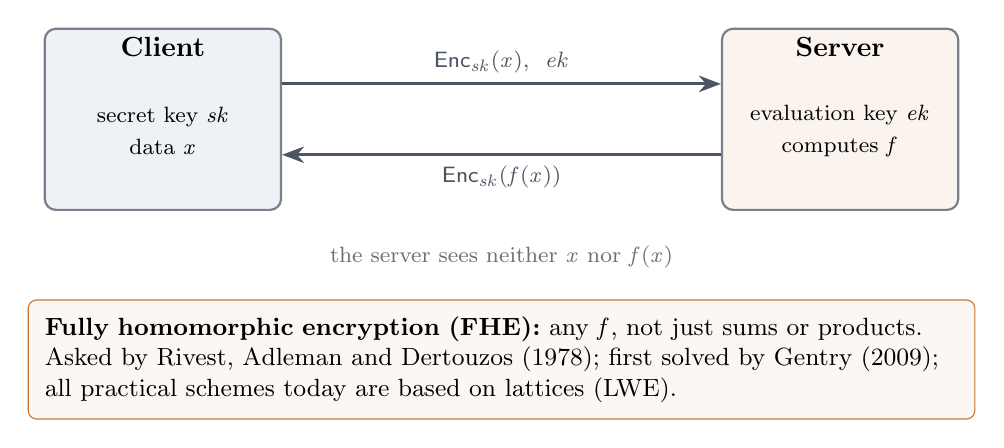
\begin{tikzpicture}[font=\small,
    msg/.style={->, line width=1.1pt, cNavy!80}]
  \node[party=cBlue!8] (client) at (0,0) {};
  \node[font=\bfseries, anchor=north] at (client.north) {Client};
  \node[align=center, font=\footnotesize] at (0,-0.15)
    {secret key $sk$\\[2pt] data $x$};
  \node[party=cOrange!8] (server) at (8.6,0) {};
  \node[font=\bfseries, anchor=north] at (server.north) {Server};
  \node[align=center, font=\footnotesize] at (8.6,-0.15)
    {evaluation key $ek$\\[2pt] computes $f$};
  \draw[msg] ([yshift=0.45cm]client.east) -- node[above, font=\footnotesize]
    {$\mathsf{Enc}_{sk}(x)$, \ $ek$} ([yshift=0.45cm]server.west);
  \draw[msg] ([yshift=-0.45cm]server.west) -- node[below, font=\footnotesize]
    {$\mathsf{Enc}_{sk}(f(x))$} ([yshift=-0.45cm]client.east);
  \node[cGray, font=\footnotesize, align=center] at (4.3,-1.75)
    {the server sees neither $x$ nor $f(x)$};
  \only<2->{
  \node[draw=cOrange, fill=cOrange!6, rounded corners=3pt, text width=11.6cm,
        align=left, font=\small, inner sep=6pt] at (4.3,-3.05)
    {\textbf{Fully homomorphic encryption (FHE):} any $f$, not just sums or
     products. Asked by Rivest, Adleman and Dertouzos (1978); first
     solved by Gentry (2009); all practical schemes today are based on
     \alert{lattices} (LWE).};}
\end{tikzpicture}
\end{frame}

%% ===========================================================================
\begin{frame}{Every lattice ciphertext carries noise}
\begin{columns}[T,onlytextwidth]
\column{0.47\textwidth}
\begin{itemize}
  \item The noise \alert{is} the security: without it, LWE is linear algebra.
  \item Homomorphic operations make it \alert{grow}; past a threshold,
        decryption fails.
  \item<2-> \textbf{Bootstrapping} (Gentry, 2009): evaluate the decryption
        homomorphically to get a \emph{fresh} ciphertext of the same message.
  \item<3-> \textbf{TFHE} (Chillotti et al., 2016/2020): bootstrap after
        \alert{every Boolean gate}, in tens of milliseconds, so circuits of
        \alert{any depth} work.
\end{itemize}
\column{0.5\textwidth}
\centering
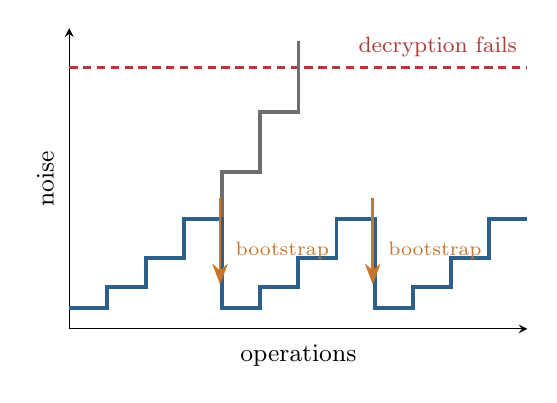
\begin{tikzpicture}
\begin{axis}[width=7.4cm, height=5.4cm, xmin=0, xmax=12, ymin=0, ymax=1.15,
    axis lines=left, xtick=\empty, ytick=\empty,
    xlabel={operations}, ylabel={noise}, label style={font=\small},
    clip=false]
  \draw[cRed, densely dashed, line width=0.9pt] (axis cs:0,1) -- (axis cs:12,1)
    node[above left, font=\footnotesize, cRed] {decryption fails};
  \addplot[cGray, line width=1.2pt, const plot, forget plot]
    coordinates {(0,0.08) (1,0.16) (2,0.27) (3,0.42) (4,0.6) (5,0.83) (6,1.1)};
  \only<2->{
  \addplot[cBlue, line width=1.4pt, const plot]
    coordinates {(0,0.08) (1,0.16) (2,0.27) (3,0.42) (4,0.08) (5,0.16) (6,0.27)
                 (7,0.42) (8,0.08) (9,0.16) (10,0.27) (11,0.42) (12,0.42)};
  \draw[->, cOrange, line width=1pt] (axis cs:3.95,0.5) -- (axis cs:3.95,0.17);
  \node[cOrange, font=\scriptsize, anchor=west] at (axis cs:4.1,0.3) {bootstrap};
  \draw[->, cOrange, line width=1pt] (axis cs:7.95,0.5) -- (axis cs:7.95,0.17);
  \node[cOrange, font=\scriptsize, anchor=west] at (axis cs:8.1,0.3) {bootstrap};}
\end{axis}
\end{tikzpicture}
\end{columns}
\end{frame}

%% ===========================================================================
\begin{frame}{This project}
\begin{columns}[T,onlytextwidth]
\column{0.5\textwidth}
\textbf{Goal} (from the proposal)
\begin{itemize}
  \item Study TFHE and implement it \alert{from scratch} in C++.
  \item Use the \alert{same parameters} as the original library
        (128-bit set: $n=630$, $N=1024$).
  \item Compare with the original on four criteria.
\end{itemize}
\vspace{6pt}
\textbf{Result}
\begin{itemize}
  \item Header-only C++17, no dependencies, \LibLines{} lines of code.
  \item 10 unit tests, one per layer; an encrypted $n$-bit adder.
\end{itemize}
\column{0.46\textwidth}
\centering
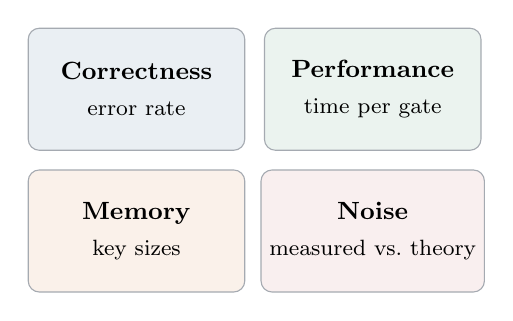
\begin{tikzpicture}[font=\small,
]
  \node[crit=cBlue!10]   at (0,0)     {\textbf{Correctness}\\[2pt]\footnotesize error rate};
  \node[crit=cGreen!10]  at (3.0,0)   {\textbf{Performance}\\[2pt]\footnotesize time per gate};
  \node[crit=cOrange!10] at (0,-1.8)  {\textbf{Memory}\\[2pt]\footnotesize key sizes};
  \node[crit=cRed!8]     at (3.0,-1.8){\textbf{Noise}\\[2pt]\footnotesize measured vs.\ theory};
\end{tikzpicture}
\end{columns}
\end{frame}

\begin{frame}{Roadmap: each concept solves a problem raised by the previous one}
\centering
\scalebox{0.93}{% The chain of concepts followed by the report (Sections 2 and 3).
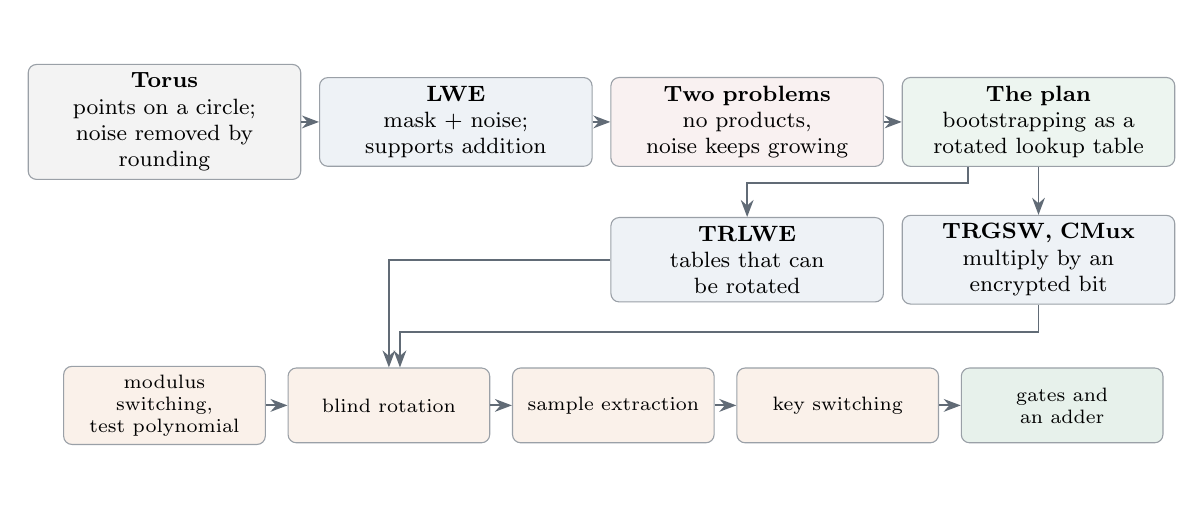
\begin{tikzpicture}[font=\footnotesize, >=Stealth,
    con/.style={draw=cNavy!45, rounded corners=3pt, align=center, inner sep=3pt,
                minimum height=1.05cm, text width=3.25cm},
    stp/.style={draw=cNavy!45, rounded corners=3pt, align=center, inner sep=3pt,
                minimum height=0.95cm, text width=2.35cm, fill=cOrange!10, font=\scriptsize},
    sec/.style={font=\scriptsize\bfseries, cGray, roadmap sec/.try},
    flow/.style={->, line width=0.7pt, cNavy!70}]
  \node[con, fill=cGray!8]  (torus) at (0,0)    {\textbf{Torus}\\points on a circle;\\noise removed by\\rounding};
  \node[con, fill=cBlue!8]  (lwe)   at (3.7,0)  {\textbf{LWE}\\mask + noise;\\supports addition};
  \node[con, fill=cRed!7]   (lim)   at (7.4,0)  {\textbf{Two problems}\\no products,\\noise keeps growing};
  \node[con, fill=cGreen!9] (plan)  at (11.1,0) {\textbf{The plan}\\bootstrapping as a\\rotated lookup table};
  \node[con, fill=cBlue!8]  (trlwe) at (7.4,-1.75)  {\textbf{TRLWE}\\tables that can\\be rotated};
  \node[con, fill=cBlue!8]  (trgsw) at (11.1,-1.75) {\textbf{TRGSW, CMux}\\multiply by an\\encrypted bit};
  \node[stp] (ms) at (0,-3.6)    {modulus switching,\\test polynomial};
  \node[stp] (br) at (2.85,-3.6) {blind rotation};
  \node[stp] (se) at (5.7,-3.6)  {sample extraction};
  \node[stp] (ks) at (8.55,-3.6) {key switching};
  \node[stp, fill=cGreen!12] (gt) at (11.4,-3.6) {gates and\\an adder};
  \draw[flow] (torus) -- (lwe);
  \draw[flow] (lwe) -- (lim);
  \draw[flow] (lim) -- (plan);
  \draw[flow] (plan.south) ++(-0.9,0) -- ++(0,-0.2) -| (trlwe.north);
  \draw[flow] (plan) -- (trgsw);
  \draw[flow] (trlwe.west) -| (br.north);
  \draw[flow] (trgsw.south) |- ++(0,-0.35) -| ([xshift=4pt]br.north);
  \draw[flow] (ms) -- (br);
  \draw[flow] (br) -- (se);
  \draw[flow] (se) -- (ks);
  \draw[flow] (ks) -- (gt);
  \node[sec, anchor=south west] at (torus.north west) {\S2.1};
  \node[sec, anchor=south west] at (lwe.north west) {\S2.2};
  \node[sec, anchor=south west] at (lim.north west) {\S2.3};
  \node[sec, anchor=south west] at (plan.north west) {\S2.4};
  \node[sec, anchor=south west] at (trlwe.north west) {\S2.5};
  \node[sec, anchor=south east] at (trgsw.north east) {\S2.6};
  \node[sec, anchor=north] at (5.7,-4.15) {\S3: one gate, step by step};
\end{tikzpicture}
}

\vspace{8pt}
\small then: \textbf{implementation} (FFT, offset trick, frequency-domain keys)
\ $\to$ \ \textbf{evaluation} (correctness, time, memory, noise)
\end{frame}

%% ===========================================================================
\section{The scheme}

\begin{frame}{The torus $\T=\R/\Z$}
\begin{columns}[c,onlytextwidth]
\column{0.42\textwidth}
\centering
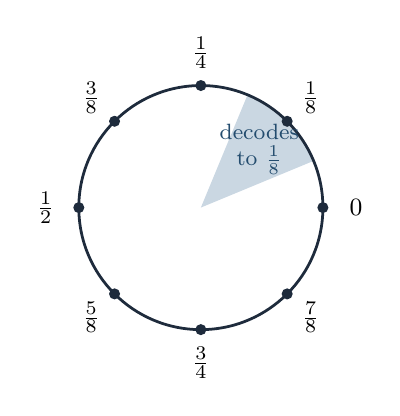
\begin{tikzpicture}[font=\small]
  \def\rad{1.55}
  \fill<2->[cBlue!25] (0,0) -- (22.5:\rad) arc (22.5:67.5:\rad) -- cycle;
  \draw[line width=1pt, cNavy] (0,0) circle (\rad);
  \foreach \k/\lab in {0/0, 1/\frac18, 2/\frac14, 3/\frac38, 4/\frac12,
                       5/\frac58, 6/\frac34, 7/\frac78} {
    \fill[cNavy] (\k*45:\rad) circle (2pt);
    \node at (\k*45:\rad+0.42) {$\lab$};
  }
  \node<2->[font=\footnotesize, align=center, cBlue!80!black] at (45:1.05)
    {decodes\\to $\frac18$};
\end{tikzpicture}
\column{0.56\textwidth}
\textbf{Why a circle?} Messages can be added, and small errors are
removed by \alert{rounding}. \muted{($0.25\equiv1.25\equiv-0.75$)}
\vspace{2pt}
\begin{itemize}
  \item A $\Z$-module: $t+t'$ and $k\cdot t$ exist, but \alert{not} $t\cdot t'$
        \muted{($\frac12\equiv\frac32$, yet $\frac12\cdot\frac12\not\equiv\frac32\cdot\frac12$)}.
  \item<2-> Message $m\in\Z_M\mapsto m/M$; decoding rounds and tolerates
        errors $<\frac1{2M}$.
\end{itemize}
\onslide<3->{
\vspace{4pt}
\begin{block}{In code: \texttt{uint32\_t}; overflow $=$ mod 1}
\centering\footnotesize
$0.75+0.5\equiv0.25$:\\ \texttt{0xC0000000 + 0x80000000} $\to$ \texttt{0x40000000}
\end{block}}
\end{columns}
\end{frame}

%% ===========================================================================
\begin{frame}{LWE: hiding a message with a mask and noise}
\begin{columns}[T,onlytextwidth]
\column{0.52\textwidth}
\textbf{First attempt:} secret bits $s\in\{0,1\}^n$, public random $\mathbf a$,
\[b=\langle\mathbf a,s\rangle+\mu\]
\muted{\small only the key owner can remove the mask $\langle\mathbf a,s\rangle$\dots}

\onslide<2->{\alert{Broken:} every ciphertext is a \emph{linear equation} in $s$;
$n$ of them $\Rightarrow$ Gaussian elimination.}

\vspace{6pt}
\onslide<3->{\textbf{Fix} (Regev 2005): make every equation slightly wrong,
\[b=\langle\mathbf a,s\rangle+\mu+\alert{e},\qquad e\sim\mathcal N(0,\sigma^2)\]
Recovering $s$ is now the \textbf{LWE problem}: believed hard, even for
quantum computers.}
\column{0.45\textwidth}
\onslide<4->{
\begin{block}{Decryption = phase, then round}
$\varphi_s(c)=b-\langle\mathbf a,s\rangle=\mu+e$\\[2pt]
\small the noise \alert{is} the security; rounding removes it
\end{block}}
\onslide<5->{
\begin{exampleblock}{Toy example: 8-bit torus, $n=4$, $\Z_4$}
\small
$s=(1,0,1,1)$, $\mathbf a=(100,37,201,54)$, $\mu=64$, $e=3$\\[2pt]
$b=355+64+3\equiv166$\\[2pt]
phase $=166-355\equiv\mathbf{67}\approx64$ $\Rightarrow$ message $1$
\end{exampleblock}}
\end{columns}
\end{frame}

%% ===========================================================================
\begin{frame}{What LWE can and cannot do}
\begin{columns}[T,onlytextwidth]
\column{0.48\textwidth}
\textbf{Can: linear operations, for free}
\begin{itemize}
  \item The phase is linear: $\varphi(c_1+c_2)=\varphi(c_1)+\varphi(c_2)$.
  \item $\frac38+\frac68\equiv\frac18$: addition mod 8 without the key.
  \item Constants via the trivial sample $(\mathbf0,\mu)$.
\end{itemize}
\onslide<2->{
\vspace{6pt}
\textbf{Cannot:}
\begin{enumerate}
  \item \alert{no products}: components are torus elements;
  \item \alert{noise grows}: variances add at every operation.
\end{enumerate}}
\column{0.48\textwidth}
\onslide<3->{
\begin{block}{TFHE's bootstrapping fixes both}
In: LWE of a noisy phase $\varphi$.\\
Out: LWE of $f(\varphi)$ with \alert{fresh} noise.\\[4pt]
For gates, $f$ = \emph{which half of the circle?}
\begin{itemize}
  \item nonlinear $\Rightarrow$ fixes 1
  \item fresh noise $\Rightarrow$ fixes 2
\end{itemize}
\end{block}}
\onslide<4->{\centering\small But how can a server compute $f(\varphi)$\\ without knowing $\varphi$?}
\end{columns}
\end{frame}

%% ===========================================================================
\begin{frame}{The plan: bootstrapping as an encrypted table lookup}
\centering
% The plan of TFHE's bootstrapping: a lookup table stored in a polynomial,
% rotated by the encrypted phase, read at position 0. Shared by report and slides.
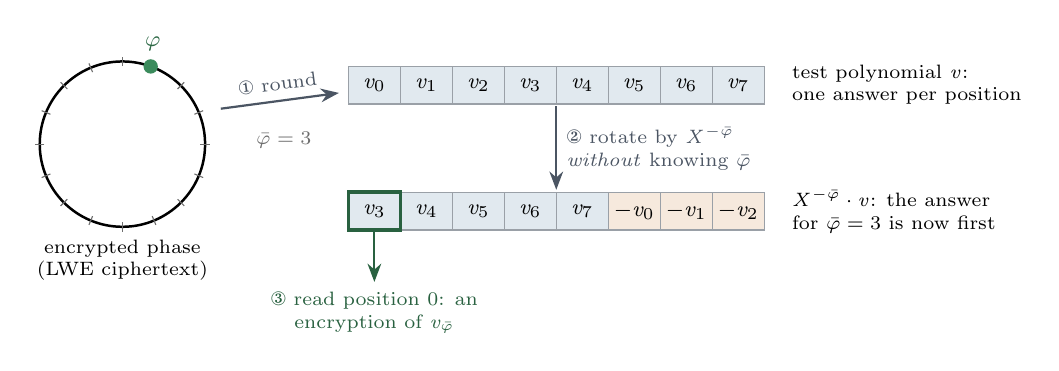
\begin{tikzpicture}[font=\footnotesize, >=Stealth]
  % ---------------- encrypted phase ----------------
  \def\rad{1.05}
  \draw[line width=0.9pt] (0,0) circle (\rad);
  \foreach \k in {0,...,15} \draw[cGray] (\k*22.5:\rad-0.06) -- (\k*22.5:\rad+0.06);
  \fill[cGreen] (70:\rad) circle (2.6pt);
  \node[cGreen!75!black, anchor=south] at (70:\rad+0.08) {$\varphi$};
  \node[align=center, font=\scriptsize] at (0,-\rad-0.42) {encrypted phase\\(LWE ciphertext)};
  % ---------------- the table ----------------
  \def\cw{0.66}
  \begin{scope}[shift={(3.2,0.75)}]
    \foreach \j in {0,...,7}
      \node[draw=cNavy!45, fill=cBlue!14, minimum width=\cw cm, minimum height=0.48cm,
            inner sep=0pt] (t\j) at (\j*\cw,0) {$v_{\j}$};
    \node[anchor=west, align=left, font=\scriptsize] at (8*\cw-0.1,0)
      {test polynomial $v$:\\one answer per position};
  \end{scope}
  \begin{scope}[shift={(3.2,-0.85)}, visible on=<3->]
    \foreach \v/\f [count=\j from 0] in {v_3/cBlue!14, v_4/cBlue!14, v_5/cBlue!14,
        v_6/cBlue!14, v_7/cBlue!14, -v_0/cOrange!16, -v_1/cOrange!16, -v_2/cOrange!16}
      \node[draw=cNavy!45, fill=\f, minimum width=\cw cm, minimum height=0.48cm,
            inner sep=0pt] (r\j) at (\j*\cw,0) {$\v$};
    \draw[cGreen!70!black, line width=1.3pt] (-0.5*\cw,-0.24) rectangle (0.5*\cw,0.24);
    \node[anchor=west, align=left, font=\scriptsize] at (8*\cw-0.1,0)
      {$X^{-\bar\varphi}\cdot v$: the answer\\for $\bar\varphi=3$ is now first};
  \end{scope}
  % ---------------- the three steps ----------------
  \draw[->, line width=0.8pt, cNavy!80, visible on=<2->] (1.25,0.45) -- node[above, sloped, font=\scriptsize] {\ding{172} round} (2.75,0.65);
  \node[visible on=<2->, font=\scriptsize, cGray] at (2.05,0.05) {$\bar\varphi=3$};
  \draw[->, line width=0.8pt, cNavy!80, visible on=<3->] (3.2+3.5*\cw,0.48) -- (3.2+3.5*\cw,-0.58)
    node[midway, right, font=\scriptsize, align=left] {\ding{173} rotate by $X^{-\bar\varphi}$\\
      \emph{without} knowing $\bar\varphi$};
  \draw[->, line width=0.8pt, cGreen!70!black, visible on=<4->] (3.2,-1.1) -- (3.2,-1.75)
    node[below, align=center, font=\scriptsize] {\ding{174} read position 0: an\\encryption of $v_{\bar\varphi}$};
\end{tikzpicture}


\vspace{4pt}
\begin{columns}[T,onlytextwidth]
\column{0.5\textwidth}
\onslide<5->{\small \textbf{Tool (a):} an encrypted table that can be rotated
\alert{cheaply and without growing noise} $\to$ \textbf{TRLWE}}
\column{0.48\textwidth}
\onslide<6->{\small \textbf{Tool (b):} rotate by a \alert{secret} amount, i.e.,
``if encrypted bit then rotate'' $\to$ \textbf{TRGSW, CMux}}
\end{columns}
\end{frame}

%% ===========================================================================
\begin{frame}{Tool (a): tables that can be rotated (polynomials and TRLWE)}
\begin{columns}[T,onlytextwidth]
\column{0.5\textwidth}
Table $=$ polynomial $v_0+v_1X+\dots$; \ rotation $=$ multiplication by $X$.\\[2pt]
\textbf{Negacyclic rotation} \muted{($X^N=-1$, exponents mod $2N$)}
\vspace{4pt}

\centering
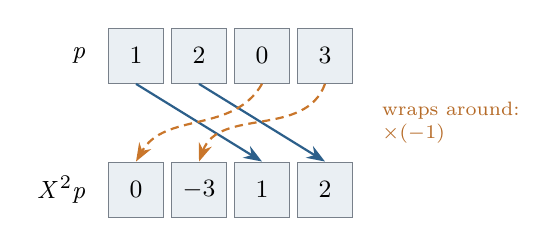
\begin{tikzpicture}[font=\small,
]
  \node[anchor=east] at (-0.5,0) {$p$};
  \foreach \v [count=\i from 0] in {1,2,0,3} \node[cellA=cBlue!10] (a\i) at (\i*0.8,0) {$\v$};
  \node[anchor=east] at (-0.5,-1.7) {$X^2p$};
  \foreach \v [count=\i from 0] in {0,-3,1,2} \node[cellA=cBlue!10] (b\i) at (\i*0.8,-1.7) {$\v$};
  \draw[->, cBlue, line width=0.8pt] (a0.south) -- (b2.north);
  \draw[->, cBlue, line width=0.8pt] (a1.south) -- (b3.north);
  \draw[->, cOrange, densely dashed, line width=0.8pt] (a3.south) to[out=-110, in=70] (b1.north);
  \draw[->, cOrange, densely dashed, line width=0.8pt] (a2.south) to[out=-120, in=60] (b0.north);
  \node[cOrange!90!black, font=\scriptsize, align=left, anchor=west] at (3.0,-0.85) {wraps around:\\$\times(-1)$};
\end{tikzpicture}

\small $(1+2X+3X^3)\cdot X^2=-3X+X^2+2X^3$
\column{0.48\textwidth}
\onslide<2->{
\begin{block}{TRLWE under $s'\in\B_N[X]$}
$c=(a,b)$, \ $b=a\cdot s'+\mu+e$ \ in $\TN$\\[2pt]
phase $b-a\cdot s'=\mu+e$: a whole polynomial
\end{block}}
\begin{itemize}
  \item<3-> Rotation for free:
        $\varphi(X^ea,X^eb)=X^e\,\varphi(c)$.
  \item<3-> Noise is only \alert{permuted}, never amplified.
  \item<3-> One sample holds a \alert{table} of $N$ values.
\end{itemize}
\end{columns}
\end{frame}

%% ===========================================================================
\begin{frame}{Tool (b): rotating by a secret amount}
The rotation depends on $\varphi=b-\sum_ia_is_i$, i.e., on the \alert{secret bits}
$s_i$. It can be done one bit at a time:
\[
  \mathrm{ACC}\gets\begin{cases}X^{k_i}\cdot\mathrm{ACC} & \text{if } s_i=1\\
                                \mathrm{ACC} & \text{if } s_i=0\end{cases}
  \;=\;\mathrm{ACC}+\alert{s_i}\cdot(X^{k_i}-1)\cdot\mathrm{ACC}
\]
\onslide<2->{\centering $\Rightarrow$ we must \textbf{multiply a TRLWE ciphertext by an encrypted bit}.\\[8pt]}
\begin{columns}[T,onlytextwidth]
\column{0.48\textwidth}
\onslide<3->{
\begin{alertblock}{Obstacle 1}
The bit cannot be an LWE/TRLWE ciphertext: torus $\times$ torus does not exist.
\end{alertblock}}
\column{0.48\textwidth}
\onslide<4->{
\begin{alertblock}{Obstacle 2}
Even $k\cdot c$ is dangerous: noise $\times|k|$, and coefficients are 32-bit numbers.
\end{alertblock}}
\end{columns}
\vspace{4pt}
\onslide<5->{\centering\small TFHE's answer in three steps: \textbf{small digits} $\to$
\textbf{precomputed encryptions (TRGSW)} $\to$ \textbf{external product}}
\end{frame}

%% ===========================================================================
\begin{frame}{Step 1: small digits instead of a big factor (gadget decomposition)}
\begin{columns}[T,onlytextwidth]
\column{0.44\textwidth}
\textbf{Removes obstacle 2:} only small integers will ever multiply a
ciphertext.

\vspace{6pt}
\textbf{Idea:} write the big factor with \alert{small digits}
\[
t\approx\frac{d_1}{\Bg}+\frac{d_2}{\Bg^2}+\dots+\frac{d_\ell}{\Bg^\ell},\qquad
d_i\in\big[-\tfrac{\Bg}{2},\tfrac{\Bg}{2}\big)
\]
with error at most $\varepsilon=1/(2\Bg^\ell)$.

\vspace{4pt}
\muted{Here: $\Bg=2^7$, $\ell=3$, digits in $[-64,64)$, $\varepsilon=2^{-22}$.}
\column{0.53\textwidth}
\centering
\textbf{The same idea in base 10}, $\ell=2$, digits in $[-5,5)$\\[8pt]
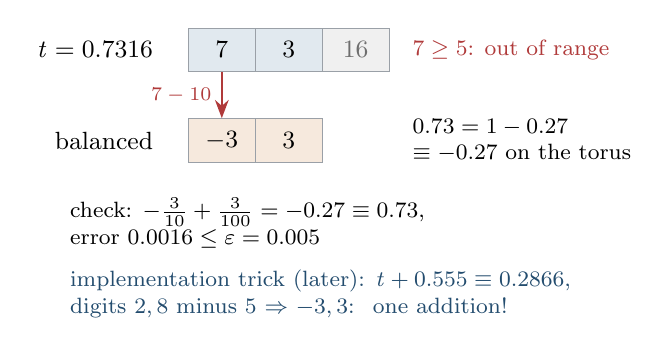
\begin{tikzpicture}[font=\small,
    dig/.style={draw=cNavy!45, minimum width=0.85cm, minimum height=0.55cm}]
  \node[anchor=east] at (-0.3,0) {$t=0.7316$};
  \node[dig, fill=cBlue!14] (a1) at (0.45,0) {$7$};
  \node[dig, fill=cBlue!14] (a2) at (1.3,0) {$3$};
  \node[dig, fill=cGray!10, text=cGray] at (2.15,0) {$16$};
  \node[visible on=<2->, anchor=west, cRed, font=\footnotesize] at (2.75,0) {$7\ge5$: out of range};
  \node[visible on=<3->, anchor=east] at (-0.3,-1.15) {balanced};
  \node[visible on=<3->, dig, fill=cOrange!16] (b1) at (0.45,-1.15) {$-3$};
  \node[visible on=<3->, dig, fill=cOrange!16] (b2) at (1.3,-1.15) {$3$};
  \node[visible on=<3->, anchor=west, font=\footnotesize, align=left] at (2.75,-1.15)
    {$0.73=1-0.27$\\$\equiv-0.27$ on the torus};
  \draw[visible on=<3->, ->, cRed, line width=0.8pt] (a1.south) -- node[left, font=\scriptsize] {$7-10$} (b1.north);
  \node[visible on=<4->, anchor=west, font=\footnotesize, align=left] at (-1.6,-2.2)
    {check: $-\frac{3}{10}+\frac{3}{100}=-0.27\equiv0.73$,\\error $0.0016\le\varepsilon=0.005$};
  \node[visible on=<5->, anchor=west, font=\footnotesize, align=left, cBlue!80!black] at (-1.6,-3.1)
    {implementation trick (later): $t+0.555\equiv0.2866$,\\
     digits $2,8$ minus $5$ $\Rightarrow$ $-3,3$: \ one addition!};
\end{tikzpicture}
\end{columns}
\end{frame}

%% ===========================================================================
\begin{frame}{Step 2: precomputed encryptions (TRGSW)}
\textbf{Goal:} an encryption of $m\cdot\varphi(d)=m\,b-m\,s'\,a$, for $d=(a,b)$
and a secret bit $m$.

\vspace{6pt}
\onslide<2->{Decompose $a\approx\sum u_i\Bg^{-i}$ and $b\approx\sum w_i\Bg^{-i}$:
the digits are \alert{public and small}, the server computes them.
\[
  m\,\varphi(d)\approx\sum_i w_i\cdot\Big(\tikz[baseline]\node[fill=cOrange!20, inner sep=2pt, rounded corners=2pt, anchor=base]{$\frac{m}{\Bg^{i}}$};\Big)
               +\sum_i u_i\cdot\Big(\tikz[baseline]\node[fill=cOrange!20, inner sep=2pt, rounded corners=2pt, anchor=base]{$\frac{-m\,s'}{\Bg^{i}}$};\Big)
\]}
\onslide<3->{The \colorbox{cOrange!20}{highlighted} terms depend on the secret: the
server receives them \alert{encrypted}.}

\vspace{6pt}
\onslide<4->{
\begin{block}{TRGSW sample of $m$}
$2\ell$ TRLWE encryptions of zero, plus $m/\Bg^{i}$ in one component:\\
row $i$ has phase $e_i-m\,s'/\Bg^{i}$, \ row $\ell+i$ has phase $e_{\ell+i}+m/\Bg^{i}$.
\ \muted{Each row is encrypted: nothing about $m$ leaks.}
\end{block}}
\end{frame}

%% ===========================================================================
\begin{frame}{Step 3: the external product}
\centering
\scalebox{0.86}{% A TRGSW sample as 2*ell TRLWE rows, and the external product as a weighted
% sum of rows by the gadget digits. Shared by the report and the slides.
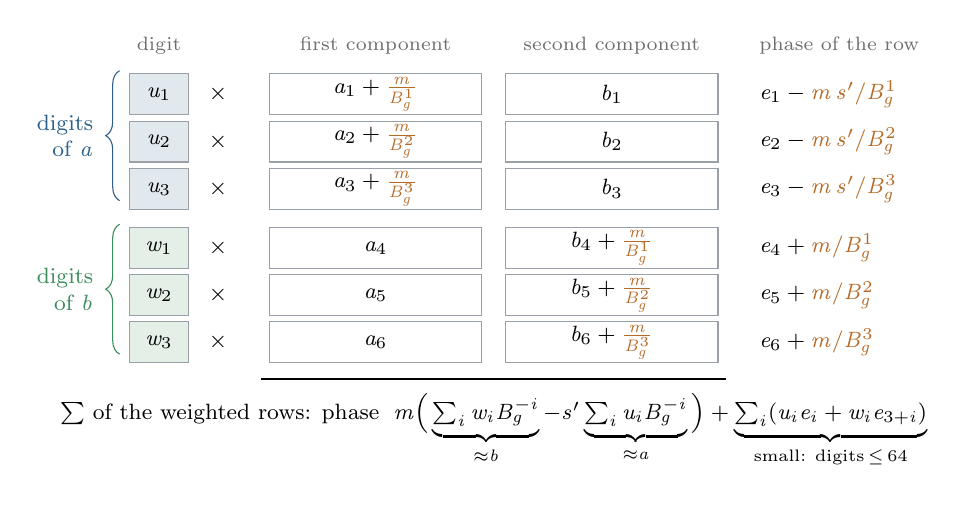
\begin{tikzpicture}[font=\footnotesize, >=Stealth,
    cell/.style={draw=cNavy!45, minimum height=0.52cm, inner sep=1pt}]
  \def\dy{0.6}
  \node[font=\scriptsize, cGray] at (0,0.62) {digit};
  \node[font=\scriptsize, cGray] at (2.75,0.62) {first component};
  \node[font=\scriptsize, cGray] at (5.75,0.62) {second component};
  \node[font=\scriptsize, cGray, anchor=west] at (7.5,0.62) {phase of the row};
  \foreach \i in {1,2,3} {
    \pgfmathsetmacro{\y}{-(\i-1)*\dy}
    \node[cell, fill=cBlue!14, minimum width=0.75cm] at (0,\y) {$u_{\i}$};
    \node at (0.75,\y) {$\times$};
    \node[cell, fill=white, minimum width=2.7cm] at (2.75,\y)
      {$a_{\i}+{\color{cOrange!90!black}\frac{m}{\Bg^{\i}}}$};
    \node[cell, fill=white, minimum width=2.7cm] at (5.75,\y) {$b_{\i}$};
    \node[anchor=west] at (7.5,\y) {$e_{\i}-{\color{cOrange!90!black}m\,s'/\Bg^{\i}}$};
  }
  \foreach \i in {1,2,3} {
    \pgfmathsetmacro{\y}{-(\i+2)*\dy-0.15}
    \pgfmathtruncatemacro{\r}{\i+3}
    \node[cell, fill=cGreen!14, minimum width=0.75cm] at (0,\y) {$w_{\i}$};
    \node at (0.75,\y) {$\times$};
    \node[cell, fill=white, minimum width=2.7cm] at (2.75,\y) {$a_{\r}$};
    \node[cell, fill=white, minimum width=2.7cm] at (5.75,\y)
      {$b_{\r}+{\color{cOrange!90!black}\frac{m}{\Bg^{\i}}}$};
    \node[anchor=west] at (7.5,\y) {$e_{\r}+{\color{cOrange!90!black}m/\Bg^{\i}}$};
  }
  \draw[decorate, decoration={brace, amplitude=5pt}, cBlue]
    (-0.5,-1.35) -- (-0.5,0.3) node[midway, left=6pt, align=right] {digits\\of $a$};
  \draw[decorate, decoration={brace, amplitude=5pt}, cGreen]
    (-0.5,-3.3) -- (-0.5,-1.65) node[midway, left=6pt, align=right] {digits\\of $b$};
  \draw[line width=0.7pt] (1.3,-3.62) -- (7.2,-3.62);
  \node[anchor=north, align=center] at (4.25,-3.68)
    {$\sum$ of the weighted rows: phase
     $\;m\Big(\underbrace{\textstyle\sum_iw_i\Bg^{-i}}_{\approx b}
       -s'\underbrace{\textstyle\sum_iu_i\Bg^{-i}}_{\approx a}\Big)
       +\underbrace{\textstyle\sum_i(u_ie_i+w_ie_{3+i})}_{\text{small: digits}\,\le\,64}$};
\end{tikzpicture}
}

\vspace{4pt}
\begin{columns}[T,onlytextwidth]
\column{0.5\textwidth}
\small Weight row $i$ by its digit and add: $\;C\ext d\approx$ encryption of
\alert{$m\cdot\varphi(d)$}.\\ No torus $\times$ torus: \alert{obstacle 1 gone}.
\column{0.46\textwidth}
\onslide<2->{
\begin{alertblock}{Noise grows additively}
\small $\mathrm{Var}\le 2\ell N\beta^2\vartheta_C+m\big((1+N)\varepsilon^2+\vartheta_d\big)$
\end{alertblock}}
\end{columns}
\end{frame}

%% ===========================================================================
\begin{frame}{CMux: an encrypted if-then-else}
\centering
\scalebox{0.92}{% CMux: (a) the encrypted multiplexer; (b) the example d0 = 1/8, d1 = 5/8.
% Shared by the report and the slides.
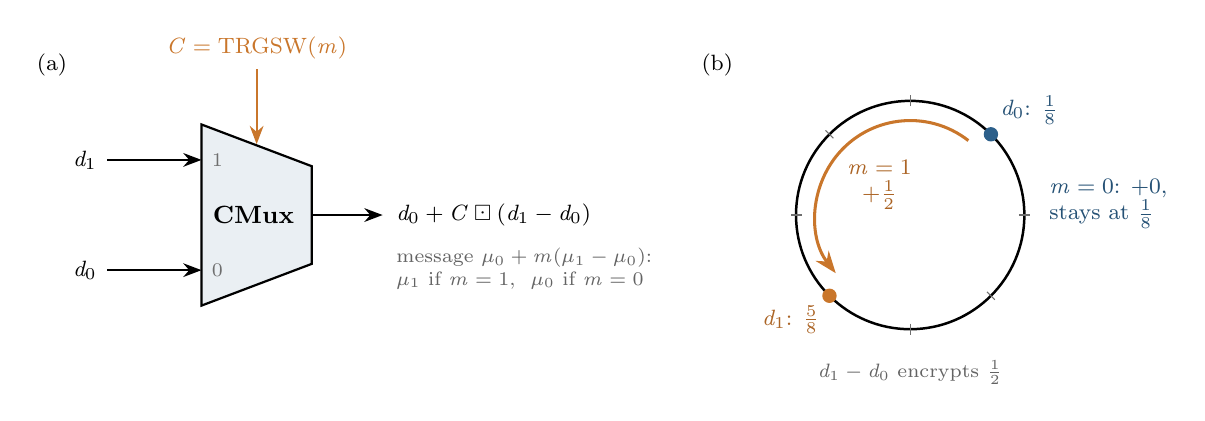
\begin{tikzpicture}[font=\footnotesize, >=Stealth]
  % ---------------- (a) ----------------
  \draw[line width=0.8pt, fill=cBlue!10] (0,-1.15) -- (0,1.15) -- (1.4,0.62) -- (1.4,-0.62) -- cycle;
  \node[font=\small\bfseries] at (0.66,0) {CMux};
  \node[font=\scriptsize, cGray] at (0.2,0.7) {1};
  \node[font=\scriptsize, cGray] at (0.2,-0.7) {0};
  \draw[->, line width=0.8pt] (-1.2,0.7) node[left] {$d_1$} -- (0,0.7);
  \draw[->, line width=0.8pt] (-1.2,-0.7) node[left] {$d_0$} -- (0,-0.7);
  \draw[->, line width=0.8pt, cOrange] (0.7,1.85) node[above] {$C=\mathrm{TRGSW}(m)$} -- (0.7,0.9);
  \draw[->, line width=0.8pt] (1.4,0) -- (2.3,0);
  \node[anchor=west, align=left] at (2.35,0) {$d_0+C\ext(d_1-d_0)$};
  \node[anchor=north west, align=left, cGray!90!black, font=\scriptsize] at (2.35,-0.3)
    {message $\mu_0+m(\mu_1-\mu_0)$:\\$\mu_1$ if $m=1$, \ $\mu_0$ if $m=0$};
  \node at (-1.9,1.9) {(a)};
  % ---------------- (b) ----------------
  \begin{scope}[xshift=9.0cm]
    \def\rad{1.45}
    \draw[line width=0.9pt] (0,0) circle (\rad);
    \foreach \k in {0,...,7} \draw[cGray] (\k*45:\rad-0.07) -- (\k*45:\rad+0.07);
    \draw[->, cOrange, line width=1.1pt, visible on=<3->] (52:\rad-0.25) arc (52:218:\rad-0.25);
    \fill[cBlue] (45:\rad) circle (2.6pt);
    \fill[cOrange] (225:\rad) circle (2.6pt);
    \node[cBlue!85!black, anchor=south west] at (45:\rad) {$d_0$: $\frac18$};
    \node[cOrange!85!black, anchor=north east] at (225:\rad) {$d_1$: $\frac58$};
    \node[cOrange!85!black, align=center, visible on=<3->] at (135:0.55)
      {$m=1$\\$+\frac12$};
    \node[cBlue!85!black, anchor=west, align=left, visible on=<2->] at (5:\rad+0.2)
      {$m=0$: $+0$,\\stays at $\frac18$};
    \node[cGray!90!black, align=center, font=\scriptsize] at (0,-\rad-0.55)
      {$d_1-d_0$ encrypts $\frac12$};
    \node at (-\rad-1.0,1.9) {(b)};
  \end{scope}
\end{tikzpicture}
}

\vspace{6pt}
\begin{columns}[T,onlytextwidth]
\column{0.5\textwidth}
\begin{itemize}
  \item One external product, \alert{the same work} for $m=0$ and $m=1$.
  \item<2-> $d_1-d_0$ encrypts $\frac12$; \ $C\ext(d_1-d_0)$ encrypts $m\cdot\frac12$.
\end{itemize}
\column{0.46\textwidth}
\onslide<4->{
\begin{exampleblock}{Exactly the step the plan needs}
\small $d_1=X^{k_i}\mathrm{ACC}$, \ $d_0=\mathrm{ACC}$, \ $C=\mathrm{TRGSW}(s_i)$\\
\muted{(\texttt{test07} checks every key bit this way)}
\end{exampleblock}}
\end{columns}
\end{frame}

%% ===========================================================================
\section{Gate bootstrapping}

\begin{frame}{Putting it together: one bootstrapped gate}
\centering
\begin{tikzpicture}[font=\small, scale=0.86, transform shape,
    stage/.style={draw=cNavy!60, rounded corners=3pt, line width=0.8pt, fill=cBlue!10,
                  minimum height=1.2cm, text width=1.55cm, align=center},
    lbl/.style={font=\scriptsize, align=center, cGray!90!black},
    kbox/.style={draw=cNavy!50, densely dashed, rounded corners=3pt, fill=cGray!8,
                 text width=3.6cm, align=center, font=\footnotesize, inner sep=4pt},
    flow/.style={->, line width=1pt, cNavy!80}]
  \node[stage, fill=cGray!6, text width=0.9cm] (in) at (0,0) {$c_1,c_2$};
  \node[stage, hl on=<2>] (lin) at (2.5,0) {linear\\combination};
  \node[stage, hl on=<3>] (br)  at (5.4,0) {blind\\rotation};
  \node[stage, hl on=<4>] (se)  at (8.3,0) {sample\\extraction};
  \node[stage, hl on=<5>] (ks)  at (11.2,0){key\\switching};
  \node[stage, fill=cGray!6, text width=0.6cm] (out) at (13.4,0) {$c$};
  \draw[flow] (in) -- node[lbl, above] {LWE} node[lbl, below] {$s,n$} (lin);
  \draw[flow] (lin) -- node[lbl, above] {LWE} node[lbl, below] {$s,n$} (br);
  \draw[flow] (br) -- node[lbl, above] {TRLWE} node[lbl, below] {$s',N$} (se);
  \draw[flow] (se) -- node[lbl, above] {LWE} node[lbl, below] {$s',N$} (ks);
  \draw[flow] (ks) -- node[lbl, above] {LWE} node[lbl, below] {$s,n$} (out);
  \node[kbox, below=1.0cm of br] (bk) {\textbf{bootstrapping key}\\$\BK_i=\mathrm{TRGSW}_{s'}(s_i)$, \ $i\le n$};
  \node[kbox, below=1.0cm of ks] (ksk) {\textbf{key-switching key}\\$\mathrm{LWE}_s(v\,s'_i/4^{j})$};
  \draw[->, densely dashed, cGray] (bk) -- (br);
  \draw[->, densely dashed, cGray] (ksk) -- (ks);
  \node[font=\small, align=left, anchor=north west, text width=13.4cm] at (0,-3.1) {%
    \only<2>{Combine the inputs so that the phase is positive $\iff$ the output is \textsf{true}. Cheap, but noises add up.}%
    \only<3>{Rotate a test polynomial by the \emph{encrypted} phase: the gate is evaluated and the noise is \alert{fresh}. $>95\%$ of the time.}%
    \only<4>{Read the constant coefficient of the TRLWE as an LWE sample under $s'$. Free, no noise.}%
    \only<5>{Bring the result back to key $s$ and dimension $n$, ready for the next gate.}};
\end{tikzpicture}
\end{frame}

%% ===========================================================================
\begin{frame}{Blind rotation: the idea}
\begin{columns}[T,onlytextwidth]
\column{0.55\textwidth}
\begin{enumerate}
  \item Round to $\Z_{2N}$: $\bar b=\round{2Nb}$, $\bar a_i=\round{2Na_i}$,
        \ $\bar\varphi=\bar b-\sum_i\bar a_is_i$.
  \item<2-> Split the rotation:
        \[X^{-\bar\varphi}=X^{-\bar b}\prod_{i=1}^{n}X^{\bar a_i s_i}\]
        each factor is $X^{\bar a_i}$ or $1$ by a \alert{secret bit}.
  \item<3-> $\mathrm{ACC}\gets(0,X^{-\bar b}v)$, then for each $i$, a CMux:
        \[\mathrm{ACC}\gets\mathrm{ACC}+\BK_i\ext\big((X^{\bar a_i}-1)\,\mathrm{ACC}\big)\]
\end{enumerate}
\column{0.42\textwidth}
\onslide<4->{
\begin{block}{Why ``blind''}
The server knows every $\bar a_i$ and $\bar b$, but not $s$:
it never learns the \alert{total rotation}.
\end{block}
\begin{block}{Cost and noise}
$n=630$ CMux $=630$ external products.\\
Fresh noise: depends on $\BK$ only.
\end{block}}
\end{columns}
\end{frame}

%% ===========================================================================
\begin{frame}{What are the $v_j$? \ \muted{\normalsize the entries of the table ($N=4$)}}
\centering
\scalebox{0.86}{% What the coefficients v_j of the test polynomial mean, for N = 4: each of the
% 2N slices of the torus is labeled with the output that the bootstrapping
% returns for phases in that slice. (a) any v; (b) the gate test polynomial;
% (c) v_j = j/8. Shared by the report and the slides.
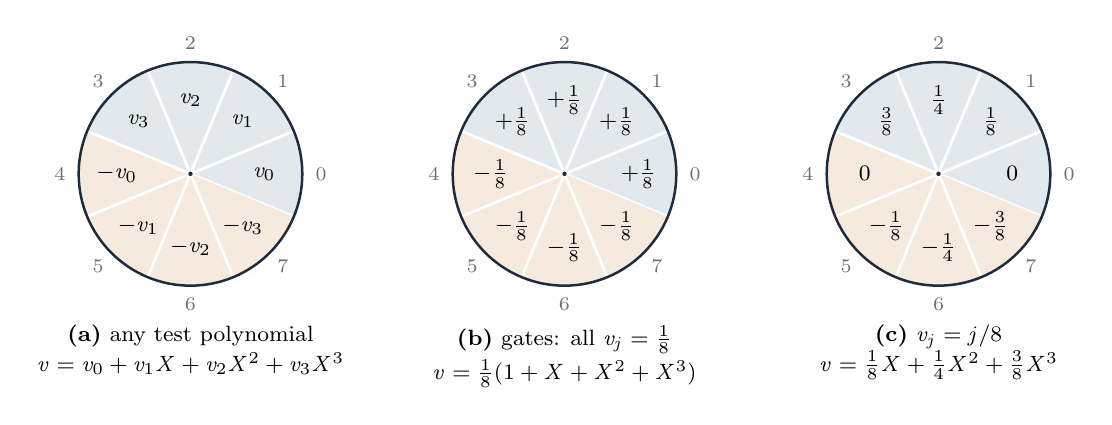
\begin{tikzpicture}[font=\footnotesize]
  \def\rad{1.42}
  % \wheel{x shift}{labels of the 8 slices}{title}{polynomial}{overlay}
  \def\wheel#1#2#3#4#5{%
    \begin{scope}[xshift=#1cm, visible on=#5]
      \foreach \lab [count=\k from 0] in {#2} {
        \pgfmathsetmacro{\aa}{\k*45-22.5}
        \pgfmathsetmacro{\bb}{\k*45+22.5}
        \ifnum\k<4
          \fill[cBlue!14] (0,0) -- (\aa:\rad) arc (\aa:\bb:\rad) -- cycle;
        \else
          \fill[cOrange!16] (0,0) -- (\aa:\rad) arc (\aa:\bb:\rad) -- cycle;
        \fi
        \draw[white, line width=1pt] (0,0) -- (\aa:\rad);
        \node at (\k*45:0.66*\rad) {\lab};
        \node[font=\scriptsize, cGray] at (\k*45:\rad+0.24) {\k};
      }
      \draw[cNavy, line width=0.9pt] (0,0) circle (\rad);
      \fill[cNavy] (0,0) circle (0.8pt);
      \node[anchor=north, align=center] at (0,-\rad-0.38) {#3\\[1pt]#4};
    \end{scope}}
  \wheel{0}{$v_0$,$v_1$,$v_2$,$v_3$,$-v_0$,$-v_1$,$-v_2$,$-v_3$}
        {\textbf{(a)} any test polynomial}{$v=v_0+v_1X+v_2X^2+v_3X^3$}{<1->}
  \wheel{4.75}{$+\frac18$,$+\frac18$,$+\frac18$,$+\frac18$,$-\frac18$,$-\frac18$,$-\frac18$,$-\frac18$}
        {\textbf{(b)} gates: all $v_j=\frac18$}{$v=\frac18(1+X+X^2+X^3)$}{<2->}
  \wheel{9.5}{$0$,$\frac18$,$\frac14$,$\frac38$,$0$,$-\frac18$,$-\frac14$,$-\frac38$}
        {\textbf{(c)} $v_j=j/8$}{$v=\frac18X+\frac14X^2+\frac38X^3$}{<3->}
\end{tikzpicture}
}

\vspace{2pt}
\begin{columns}[T,onlytextwidth]
\column{0.5\textwidth}
\small
\begin{itemize}
  \item $v_j$ \textbf{is the output} for slice $\bar\varphi=j$, i.e., for phases close to $j/(2N)$.
  \item Slice $N+j$ (opposite) returns \alert{$-v_j$}, because $X^N=-1$.
\end{itemize}
\column{0.47\textwidth}
\small
\begin{itemize}
  \item To evaluate $f$: \alert{$v_j=f\big(j/(2N)\big)$}.
  \item<2-> Gates: all $v_j=\frac18$ $\Rightarrow$ sign.
  \item<3-> $v_j=j/8$: returns the rounded phase.
\end{itemize}
\end{columns}
\end{frame}

%% ===========================================================================
\begin{frame}{The test polynomial is a lookup table \ \muted{\normalsize($N=4$)}}
\centering
% The test polynomial as a lookup table, for N = 4: (a) the 2N positions of the
% rounded phase on the torus; (b) X^(-phibar) * v for every phibar, whose
% constant coefficient (framed) is the output. Shared by the report and slides.
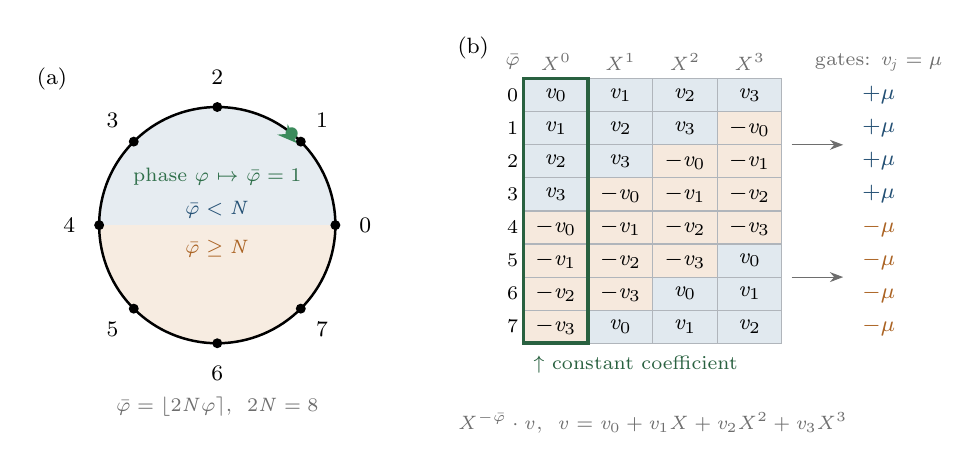
\begin{tikzpicture}[font=\footnotesize, >=Stealth]
  % ---------------- (a) ----------------
  \begin{scope}
    \def\rad{1.5}
    \fill[cBlue!12] (0,0) -- (\rad,0) arc (0:180:\rad) -- cycle;
    \fill[cOrange!14] (0,0) -- (-\rad,0) arc (180:360:\rad) -- cycle;
    \draw[line width=0.9pt] (0,0) circle (\rad);
    \foreach \p in {0,...,7} {
      \fill (\p*45:\rad) circle (1.8pt);
      \node at (\p*45:\rad+0.38) {$\p$};
    }
    \fill[cGreen] (51:\rad) circle (2.2pt);
    \draw[->, cGreen, line width=0.9pt] (51:\rad-0.05) arc (51:46:\rad-0.05);
    \node[cGreen!80!black, align=center, font=\scriptsize] at (0,0.62)
      {phase $\varphi$ $\mapsto$ $\bar\varphi=1$};
    \node[cBlue!85!black, font=\scriptsize] at (0,0.2) {$\bar\varphi<N$};
    \node[cOrange!85!black, font=\scriptsize] at (0,-0.3) {$\bar\varphi\ge N$};
    \node[align=center, font=\scriptsize, cGray] at (0,-\rad-0.8) {$\bar\varphi=\round{2N\varphi}$, \ $2N=8$};
    \node at (-\rad-0.6,\rad+0.35) {(a)};
  \end{scope}
  % ---------------- (b) ----------------
  \begin{scope}[xshift=4.3cm, yshift=1.65cm]
    \def\cw{0.82}
    \def\ch{0.42}
    \node[font=\scriptsize, cGray] at (-0.55,0.42) {$\bar\varphi$};
    \foreach \j in {0,...,3}
      \node[font=\scriptsize, cGray] at (\j*\cw,0.42) {$X^{\j}$};
    \foreach \r in {0,...,7} {
      \node[font=\scriptsize] at (-0.55,-\r*\ch) {\r};
      \foreach \j in {0,...,3} {
        \pgfmathtruncatemacro{\k}{\j+\r}
        \pgfmathtruncatemacro{\q}{mod(floor(\k/4),2)}
        \pgfmathtruncatemacro{\c}{mod(\k,4)}
        \ifnum\q=0
          \node[draw=cNavy!35, fill=cBlue!14, minimum width=\cw cm, minimum height=\ch cm,
                inner sep=0pt] at (\j*\cw,-\r*\ch) {$v_{\c}$};
        \else
          \node[draw=cNavy!35, fill=cOrange!16, minimum width=\cw cm, minimum height=\ch cm,
                inner sep=0pt] at (\j*\cw,-\r*\ch) {$-v_{\c}$};
        \fi
      }
    }
    \draw[cGreen!70!black, line width=1.3pt] (-0.5*\cw,0.5*\ch) rectangle (0.5*\cw,-7.5*\ch);
    \node[cGreen!70!black, font=\scriptsize, anchor=north west] at (-0.5*\cw,-7.6*\ch)
      {$\uparrow$ constant coefficient};
    \node[font=\scriptsize, align=center, cGray] at (1.5*\cw,-9.9*\ch)
      {$X^{-\bar\varphi}\cdot v$, \ $v=v_0+v_1X+v_2X^2+v_3X^3$};
    % output with the gate test polynomial
    \begin{scope}[visible on=<2->]
      \node[font=\scriptsize, cGray, align=center] at (5.0*\cw,0.42) {gates: $v_j=\mu$};
      \foreach \r in {0,...,3}
        \node[cBlue!85!black] at (5.0*\cw,-\r*\ch) {$+\mu$};
      \foreach \r in {4,...,7}
        \node[cOrange!85!black] at (5.0*\cw,-\r*\ch) {$-\mu$};
      \draw[->, cGray] (3.65*\cw,-1.5*\ch) -- (4.45*\cw,-1.5*\ch);
      \draw[->, cGray] (3.65*\cw,-5.5*\ch) -- (4.45*\cw,-5.5*\ch);
    \end{scope}
    \node at (-1.05,0.6) {(b)};
  \end{scope}
\end{tikzpicture}


\vspace{4pt}
\small Rotating by $X^{-\bar\varphi}$ brings entry $v_{\bar\varphi}$ to the front: each row is
the previous one shifted left, and the coefficient that leaves \alert{comes back negated} ($X^N=-1$). \onslide<3->{\muted{Other $v$ $\Rightarrow$ other functions
(programmable bootstrapping; \texttt{test08} evaluates a 4-entry table).}}
\end{frame}

%% ===========================================================================
\begin{frame}{How the test polynomial is built, and is it encrypted?}
\begin{columns}[T,onlytextwidth]
\column{0.5\textwidth}
\textbf{Built by the server}, from the function:\\
coefficient $j$ $=$ answer for slice $\bar\varphi=j$.
\begin{itemize}
  \item Gates: all $N=1024$ coefficients $=\mu=\frac18$ \muted{(\texttt{0x20000000})}:\\
        \texttt{\footnotesize TorusPoly testv(N, MU);}
\end{itemize}
\column{0.47\textwidth}
\onslide<2->{
\begin{alertblock}{Not encrypted: it is public}
The function is no secret (``compute a NAND''). What is secret is the input,
i.e., \emph{which} entry gets selected.
\end{alertblock}}
\end{columns}
\vspace{6pt}
\centering
\onslide<2->{\scalebox{0.88}{% The test polynomial enters blind rotation as a trivial (public, noiseless)
% TRLWE sample; the first CMux turns the accumulator into a real ciphertext.
% Example of Section 3 (N = 4, b-bar = 6). Shared by the report and the slides.
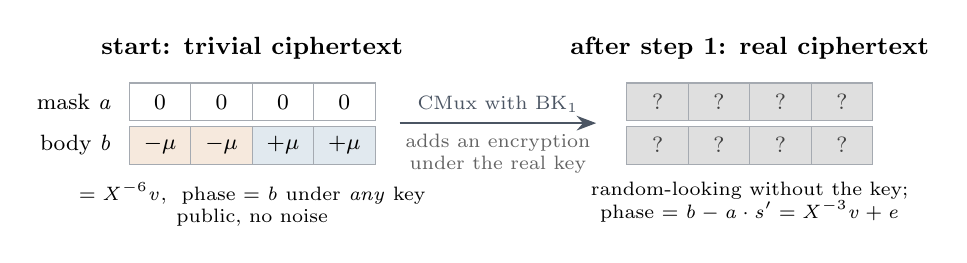
\begin{tikzpicture}[font=\footnotesize, >=Stealth]
  \def\cw{0.78}
  \def\ch{0.48}
  % ---------------- trivial sample ----------------
  \node[font=\small\bfseries, anchor=south] at (1.5*\cw,0.62) {start: trivial ciphertext};
  \node[anchor=east] at (-0.5*\cw-0.1,0.2) {mask $a$};
  \node[anchor=east] at (-0.5*\cw-0.1,-0.35) {body $b$};
  \foreach \j in {0,...,3}
    \node[draw=cNavy!40, fill=white, minimum width=\cw cm, minimum height=\ch cm,
          inner sep=0pt] at (\j*\cw,0.2) {$0$};
  \foreach \v/\f [count=\j from 0] in {-\mu/cOrange!16, -\mu/cOrange!16, +\mu/cBlue!14, +\mu/cBlue!14}
    \node[draw=cNavy!40, fill=\f, minimum width=\cw cm, minimum height=\ch cm,
          inner sep=0pt] at (\j*\cw,-0.35) {$\v$};
  \node[anchor=north, align=center, font=\scriptsize] at (1.5*\cw,-0.7)
    {$=X^{-6}v$, \ phase $=b$ under \emph{any} key\\public, no noise};
  % ---------------- the CMux ----------------
  \draw[->, line width=0.9pt, cNavy!80, visible on=<2->] (3.9*\cw,-0.07) -- (7.1*\cw,-0.07)
    node[midway, above, align=center, font=\scriptsize] {CMux with $\BK_1$}
    node[midway, below, align=center, font=\scriptsize, cGray!90!black]
      {adds an encryption\\under the real key};
  % ---------------- real ciphertext ----------------
  \begin{scope}[xshift=8.1*\cw cm, visible on=<2->]
    \node[font=\small\bfseries, anchor=south] at (1.5*\cw,0.62) {after step 1: real ciphertext};
    \foreach \j in {0,...,3}
      \node[draw=cNavy!40, fill=cGray!22, minimum width=\cw cm, minimum height=\ch cm,
            inner sep=0pt, text=cGray!60!black] at (\j*\cw,0.2) {$?$};
    \foreach \j in {0,...,3}
      \node[draw=cNavy!40, fill=cGray!22, minimum width=\cw cm, minimum height=\ch cm,
            inner sep=0pt, text=cGray!60!black] at (\j*\cw,-0.35) {$?$};
    \node[anchor=north, align=center, font=\scriptsize] at (1.5*\cw,-0.7)
      {random-looking without the key;\\phase $=b-a\cdot s'=X^{-3}v+e$};
  \end{scope}
\end{tikzpicture}
}}

\vspace{2pt}
\onslide<3->{\small Start: \textbf{trivial} sample $(0,X^{-\bar b}v)$, public since $\bar b$ is public.
After the first CMux: a \alert{real ciphertext} \ $\Rightarrow$ \ \textbf{public table, secret selection}.}
\end{frame}

%% ===========================================================================
\begin{frame}{Blind rotation, step by step \ \muted{\normalsize($n=3$, $N=4$)}}
\begin{columns}[c,onlytextwidth]
\column{0.2\textwidth}
\small
\textbf{Secret:} $s=(1,0,1)$\\[6pt]
\textbf{Public:} $\bar b=6$,\\ $\bar{\mathbf a}=(3,5,2)$\\[6pt]
\textbf{Goal:} $v_{\bar\varphi}$ without knowing $\bar\varphi$
\column{0.78\textwidth}
\centering
\scalebox{0.92}{% Blind rotation step by step, for n = 3 and N = 4. Shared by the report and
% the slides (each step appears on its own overlay in the slides).
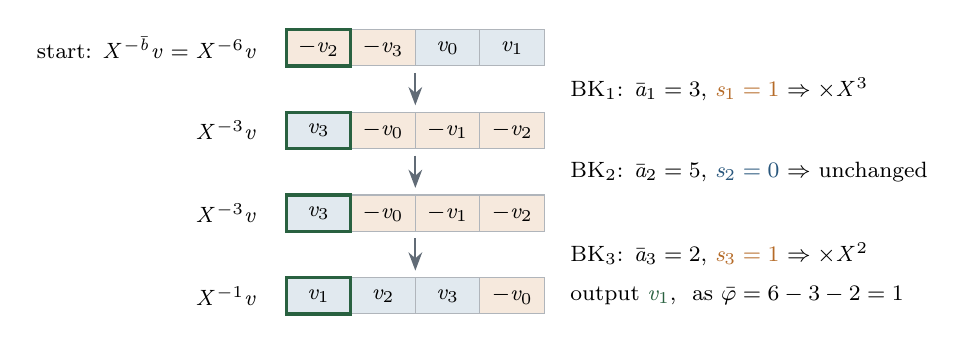
\begin{tikzpicture}[font=\footnotesize, >=Stealth]
  \def\cw{0.82}
  \def\ch{0.46}
  \def\dy{1.05}
  % one accumulator: \acc{row}{sign/index list}{overlay}; b = +v_index, o = -v_index
  \def\acc#1#2#3{%
    \begin{scope}[shift={(0,-#1*\dy)}, visible on=#3]
      \foreach \s/\c [count=\j from 0] in {#2} {
        \if\s b
          \node[draw=cNavy!35, fill=cBlue!14, minimum width=\cw cm, minimum height=\ch cm,
                inner sep=0pt] at (\j*\cw,0) {$v_{\c}$};
        \else
          \node[draw=cNavy!35, fill=cOrange!16, minimum width=\cw cm, minimum height=\ch cm,
                inner sep=0pt] at (\j*\cw,0) {$-v_{\c}$};
        \fi
      }
      \draw[cGreen!70!black, line width=1.2pt] (-0.5*\cw,-0.5*\ch) rectangle (0.5*\cw,0.5*\ch);
    \end{scope}}
  \acc{0}{o/2, o/3, b/0, b/1}{<1->}
  \acc{1}{b/3, o/0, o/1, o/2}{<2->}
  \acc{2}{b/3, o/0, o/1, o/2}{<3->}
  \acc{3}{b/1, b/2, b/3, o/0}{<4->}
  % left labels
  \begin{scope}[every node/.style={anchor=east, font=\footnotesize}]
    \node at (-0.65,0) {start: $X^{-\bar b}v=X^{-6}v$};
    \node[visible on=<2->] at (-0.65,-1*\dy) {$X^{-3}v$};
    \node[visible on=<3->] at (-0.65,-2*\dy) {$X^{-3}v$};
    \node[visible on=<4->] at (-0.65,-3*\dy) {$X^{-1}v$};
  \end{scope}
  % steps
  \begin{scope}[every node/.style={anchor=west, font=\footnotesize, align=left}]
    \draw[->, cNavy!70, line width=0.8pt, visible on=<2->] (1.5*\cw,-0.32) -- (1.5*\cw,-1*\dy+0.32);
    \node[visible on=<2->] at (3.75*\cw,-0.5*\dy)
      {$\BK_1$: $\bar a_1=3$, ${\color{cOrange!90!black}s_1=1}$ $\Rightarrow\times X^{3}$};
    \draw[->, cNavy!70, line width=0.8pt, visible on=<3->] (1.5*\cw,-1*\dy-0.32) -- (1.5*\cw,-2*\dy+0.32);
    \node[visible on=<3->] at (3.75*\cw,-1.5*\dy)
      {$\BK_2$: $\bar a_2=5$, ${\color{cBlue!90!black}s_2=0}$ $\Rightarrow$ unchanged};
    \draw[->, cNavy!70, line width=0.8pt, visible on=<4->] (1.5*\cw,-2*\dy-0.32) -- (1.5*\cw,-3*\dy+0.32);
    \node[visible on=<4->] at (3.75*\cw,-2.5*\dy)
      {$\BK_3$: $\bar a_3=2$, ${\color{cOrange!90!black}s_3=1}$ $\Rightarrow\times X^{2}$};
  \end{scope}
  \node[visible on=<5->, anchor=west, font=\footnotesize] at (3.75*\cw,-3*\dy)
    {output ${\color{cGreen!70!black}v_1}$, \ as $\bar\varphi=6-3-2=1$};
\end{tikzpicture}
}
\end{columns}
\end{frame}

%% ===========================================================================
\begin{frame}{The same run with numbers: bootstrapping an encryption of \textsf{true}}
\newcommand{\pmu}{{\color{cBlue}+\mu}}
\newcommand{\mmu}{{\color{cOrange!90!black}-\mu}}
\begin{columns}[T,onlytextwidth]
\column{0.42\textwidth}
\small
\textbf{Input:} LWE of \textsf{true} ($+\frac18$),\\ $s=(1,0,1)$, error $e=0.003$\\[3pt]
$\mathbf a=(0.37,\,0.61,\,0.24)$\\
$b=0.37+0.24+0.125+0.003=0.738$\\[6pt]
\onslide<2->{\textbf{Modulus switching} ($\times8$, round):\\
$\bar b=\round{5.904}=6$\\
$\bar{\mathbf a}=(\round{2.96},\round{4.88},\round{1.92})=(3,5,2)$\\[3pt]
$\bar\varphi=6-3-2=1$ \ \muted{(unknown to the server)}\\[6pt]}
\onslide<3->{\textbf{Gate test polynomial:} $v=[\mu,\mu,\mu,\mu]$}
\column{0.55\textwidth}
\small
\onslide<3->{
\setlength{\tabcolsep}{4pt}
\begin{tabular}{@{}lccc@{}}
\toprule
step & $\bar a_i,\,s_i$ & message of ACC & coefficients\\
\midrule
start & -- & $X^{-6}v$ \muted{(trivial)} & $[\mmu,\mmu,\pmu,\pmu]$\\
\uncover<4->{$i=1$} & \uncover<4->{$3,\ 1$} & \uncover<4->{$X^{-3}v$} & \uncover<4->{$[\pmu,\mmu,\mmu,\mmu]$}\\
\uncover<5->{$i=2$} & \uncover<5->{$5,\ 0$} & \uncover<5->{$X^{-3}v$} & \uncover<5->{$[\pmu,\mmu,\mmu,\mmu]$}\\
\uncover<6->{$i=3$} & \uncover<6->{$2,\ 1$} & \uncover<6->{$X^{-1}v$} & \uncover<6->{$[\pmu,\pmu,\pmu,\mmu]$}\\
\bottomrule
\end{tabular}\\[4pt]
\muted{\footnotesize $X^{-6}=X^2$: \ $X^2v=\mu(X^2+X^3+X^4+X^5)=\mu(-1-X+X^2+X^3)$}}

\vspace{8pt}
\onslide<7->{
\begin{exampleblock}{Sample extraction}
constant coefficient $+\mu=+\frac18$ $\Rightarrow$ \textsf{true}, with fresh noise.\\
\muted{any $\bar\varphi\in\{0,..,3\}$ gives $+\mu$; \ $\{4,..,7\}$ gives $-\mu$}
\end{exampleblock}}
\end{columns}
\end{frame}

%% ===========================================================================
\begin{frame}{Sample extraction \ \muted{\normalsize($N=4$)}}
\centering
% Sample extraction for N = 4: the constant coefficient of a * s' is the inner
% product of s' with a rearranged and partly negated copy of a.
% Shared by the report and the slides.
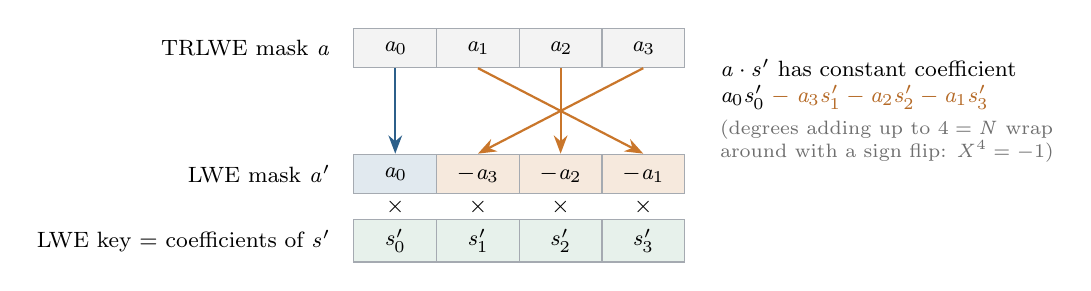
\begin{tikzpicture}[font=\footnotesize, >=Stealth]
  \def\cw{1.05}
  \def\ch{0.5}
  \foreach \v [count=\j from 0] in {a_0,a_1,a_2,a_3}
    \node[draw=cNavy!40, fill=cGray!8, minimum width=\cw cm, minimum height=\ch cm] (a\j) at (\j*\cw,0) {$\v$};
  \foreach \v/\f [count=\j from 0] in {a_0/cBlue!14,-a_3/cOrange!16,-a_2/cOrange!16,-a_1/cOrange!16}
    \node[draw=cNavy!40, fill=\f, minimum width=\cw cm, minimum height=\ch cm] (e\j) at (\j*\cw,-1.6) {$\v$};
  \foreach \v [count=\j from 0] in {s'_0,s'_1,s'_2,s'_3}
    \node[draw=cNavy!40, fill=cGreen!12, minimum width=\cw cm, minimum height=\ch cm] (s\j) at (\j*\cw,-2.45) {$\v$};
  \draw[->, cBlue, line width=0.8pt] (a0.south) -- (e0.north);
  \draw[->, cOrange, line width=0.8pt] (a3.south) -- (e1.north);
  \draw[->, cOrange, line width=0.8pt] (a2.south) -- (e2.north);
  \draw[->, cOrange, line width=0.8pt] (a1.south) -- (e3.north);
  \node[anchor=east] at (-0.7,0) {TRLWE mask $a$};
  \node[anchor=east] at (-0.7,-1.6) {LWE mask $a'$};
  \node[anchor=east] at (-0.7,-2.45) {LWE key $=$ coefficients of $s'$};
  \foreach \j in {0,...,3} \node at (\j*\cw,-2.02) {$\times$};
  \node[anchor=west, align=left] at (4*\cw-0.2,-0.8)
    {$a\cdot s'$ has constant coefficient\\
     $a_0s'_0\;{\color{cOrange!90!black}-\;a_3s'_1-a_2s'_2-a_1s'_3}$\\[2pt]
     \scriptsize\color{cGray} (degrees adding up to $4=N$ wrap\\[-1pt]
     \scriptsize\color{cGray} around with a sign flip: $X^4=-1$)};
\end{tikzpicture}


\vspace{10pt}
\begin{itemize}
  \item \textbf{Why:} blind rotation gives a TRLWE (a whole table); the next
        gate needs \alert{one LWE} sample of position $0$.
  \item Reorder and negate the mask: an LWE sample of dimension $N$, under the
        coefficients of $s'$. \alert{No arithmetic, no noise.}
\end{itemize}
\end{frame}

%% ===========================================================================
\begin{frame}{Key switching: from $s'$ ($N=1024$) back to $s$ ($n=630$)}
\centering
\scalebox{0.95}{% Key switching: one slice (fixed coefficient i) of the key-switching table and
% the entries selected by the digits of a_i = 0.7. Shared by report and slides.
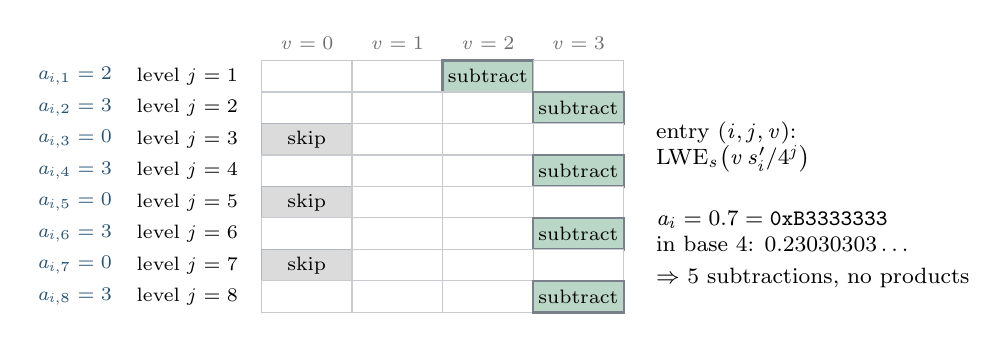
\begin{tikzpicture}[font=\footnotesize, >=Stealth]
  \def\cw{1.15}
  \def\ch{0.4}
  \foreach \v in {0,...,3} \node[font=\scriptsize, cGray] at (\v*\cw,0.42) {$v=\v$};
  \foreach \d [count=\j] in {2,3,0,3,0,3,0,3} {
    \node[font=\scriptsize, anchor=east] at (-0.75,-\j*\ch+\ch) {level $j=\j$};
    \node[font=\scriptsize, anchor=east, cBlue!85!black] at (-2.35,-\j*\ch+\ch) {$a_{i,\j}=\d$};
    \foreach \v in {0,...,3} {
      \ifnum\v=\d
        \ifnum\d=0
          \node[draw=cNavy!35, fill=cGray!25, minimum width=\cw cm, minimum height=\ch cm,
                inner sep=0pt, font=\scriptsize] at (\v*\cw,-\j*\ch+\ch) {skip};
        \else
          \node[draw=cNavy!60, fill=cGreen!35, minimum width=\cw cm, minimum height=\ch cm,
                inner sep=0pt, font=\scriptsize, line width=0.8pt] at (\v*\cw,-\j*\ch+\ch) {subtract};
        \fi
      \else
        \node[draw=cNavy!25, fill=white, minimum width=\cw cm, minimum height=\ch cm,
              inner sep=0pt] at (\v*\cw,-\j*\ch+\ch) {};
      \fi
    }
  }
  \node[anchor=west, align=left] at (3.75*\cw,-0.9)
    {entry $(i,j,v)$:\\$\mathrm{LWE}_s\big(v\,s'_i/4^{j}\big)$};
  \node[anchor=west, align=left] at (3.75*\cw,-2.2)
    {$a_i=0.7=\texttt{0xB3333333}$\\in base 4: $0.23030303\ldots$\\[2pt]
     $\Rightarrow$ 5 subtractions, no products};
\end{tikzpicture}
}

\vspace{8pt}
\begin{columns}[T,onlytextwidth]
\column{0.48\textwidth}
\begin{itemize}
  \item \textbf{Why:} the extracted sample is under $s'$ (size $1024$); gates
        expect $s$ (size $630$).
  \item The base-4 digits of each $a_i$ select table entries.
\end{itemize}
\column{0.48\textwidth}
\begin{itemize}
  \item $c'=(\mathbf0,b)-\sum_{i,j}\KSK_{i,j,a_{ij}}$: same phase, now under $s$.
  \item \alert{No multiplications}: memory (79\,MiB) for time.
\end{itemize}
\end{columns}
\end{frame}

%% ===========================================================================
\begin{frame}{Bootstrapping resets the noise}
\centering
% Bootstrapping resets the noise: a deliberately noisy encryption of +1/8 and
% the output of its bootstrapping (unit test test09). Shared by report and slides.
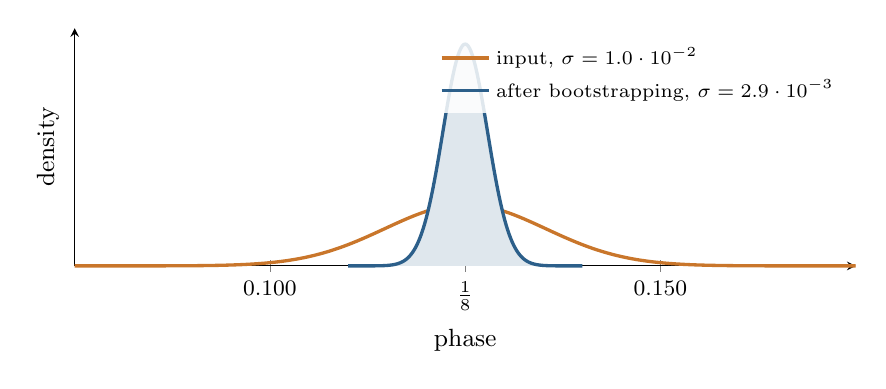
\begin{tikzpicture}
\begin{axis}[width=11.5cm, height=4.6cm, xmin=0.075, xmax=0.175, ymin=0, ymax=150,
    axis lines=left, xlabel={phase}, ylabel={density},
    xtick={0.1,0.125,0.15}, xticklabels={$0.100$,$\frac18$,$0.150$},
    ytick=\empty, tick label style={font=\footnotesize}, label style={font=\small},
    legend style={font=\scriptsize, at={(0.99,0.97)}, anchor=north east, draw=none,
                  fill=white, fill opacity=0.85, text opacity=1},
    legend cell align=left, clip=false]
  \addplot[cOrange, line width=1.2pt, domain=0.075:0.175, samples=161]
    {exp(-(x-0.125)^2/(2*\BootSdInRaw^2))/(\BootSdInRaw*sqrt(2*pi))};
  \addlegendentry{input, $\sigma=\BootSdIn$}
  \addplot[cBlue, line width=1.2pt, fill=cBlue!15, domain=0.11:0.14, samples=161, visible on=<2->]
    {exp(-(x-0.125)^2/(2*\BootSdOutRaw^2))/(\BootSdOutRaw*sqrt(2*pi))};
  \addlegendentry{after bootstrapping, $\sigma=\BootSdOut$}
\end{axis}
\end{tikzpicture}


\vspace{6pt}
\onslide<3->{
\begin{alertblock}{The key property}
The output noise depends only on the evaluation key, \textbf{not} on the input
noise ($\vartheta_{\mathrm{out}}\le\BoundTotal$): gates can be chained
\alert{forever}. \muted{(\texttt{test09}: inputs $300\times$ noisier than fresh ones)}
\end{alertblock}}
\end{frame}

%% ===========================================================================
\begin{frame}{Homomorphic gates}
\begin{columns}[c,onlytextwidth]
\column{0.5\textwidth}
\centering
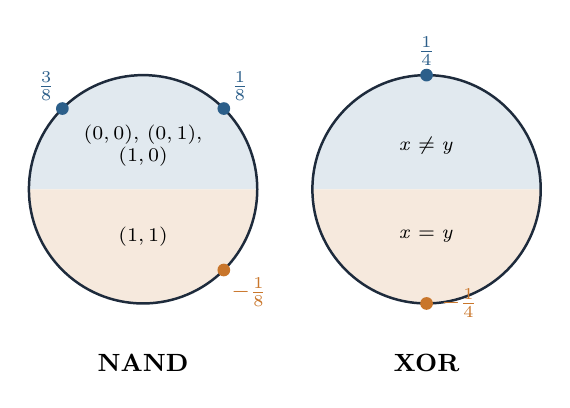
\begin{tikzpicture}[font=\footnotesize]
  \def\rad{1.45}
  \begin{scope}
    \fill[cBlue!14] (0,0) -- (\rad,0) arc (0:180:\rad) -- cycle;
    \fill[cOrange!16] (0,0) -- (-\rad,0) arc (180:360:\rad) -- cycle;
    \draw[line width=0.9pt, cNavy] (0,0) circle (\rad);
    \fill[cBlue] (135:\rad) circle (2.3pt) node[above left=-1pt] {$\frac38$};
    \fill[cBlue] (45:\rad) circle (2.3pt) node[above right=-1pt] {$\frac18$};
    \fill[cOrange] (-45:\rad) circle (2.3pt) node[below right=-1pt] {$-\frac18$};
    \node[font=\scriptsize, align=center] at (0,0.55) {$(0,0)$, $(0,1)$,\\$(1,0)$};
    \node[font=\scriptsize] at (0,-0.6) {$(1,1)$};
    \node[font=\small\bfseries] at (0,-\rad-0.75) {NAND};
  \end{scope}
  \begin{scope}[xshift=3.6cm]
    \fill[cBlue!14] (0,0) -- (\rad,0) arc (0:180:\rad) -- cycle;
    \fill[cOrange!16] (0,0) -- (-\rad,0) arc (180:360:\rad) -- cycle;
    \draw[line width=0.9pt, cNavy] (0,0) circle (\rad);
    \fill[cBlue] (90:\rad) circle (2.3pt) node[above] {$\frac14$};
    \fill[cOrange] (-90:\rad) circle (2.3pt) node[right=2pt] {$-\frac14$};
    \node[font=\scriptsize] at (0,0.55) {$x\neq y$};
    \node[font=\scriptsize] at (0,-0.6) {$x=y$};
    \node[font=\small\bfseries] at (0,-\rad-0.75) {XOR};
  \end{scope}
\end{tikzpicture}
\column{0.48\textwidth}
Bits are $\pm\frac18$. A gate = \alert{linear combination} whose phase is
positive iff the output is true, then bootstrap:
\vspace{4pt}

\small
\begin{tabular}{@{}lll@{}}
\toprule
Gate & Combination & Margin\\
\midrule
NAND & $(\mathbf0,\frac18)-c_x-c_y$ & $\frac18$\\
AND & $(\mathbf0,-\frac18)+c_x+c_y$ & $\frac18$\\
OR & $(\mathbf0,\frac18)+c_x+c_y$ & $\frac18$\\
XOR & $(\mathbf0,\frac14)+2(c_x+c_y)$ & $\frac14$\\
NOT & $-c_x$ \muted{(free)} & ---\\
\bottomrule
\end{tabular}
\end{columns}
\vspace{4pt}
\onslide<2->{\small \textbf{XOR trick:} doubling sends both equal-input cases to $\pm\frac12$, the same torus point.}
\end{frame}

%% ===========================================================================
\begin{frame}{MUX with a single key switching}
\begin{columns}[T,onlytextwidth]
\column{0.4\textwidth}
$\mathrm{MUX}(s,x,y)=(s\wedge x)\vee(\neg s\wedge y)$
\begin{itemize}
  \item Naively: 3 bootstrappings.
  \item The two ANDs are \alert{never both true} $\Rightarrow$ OR $=$ sum.
  \item<2-> 2 blind rotations (no key switching), add, $+\frac18$,
        \alert{one} key switching.
\end{itemize}
\column{0.57\textwidth}
\onslide<2->{
\centering\small
\setlength{\tabcolsep}{4pt}
\begin{tabular}{@{}ccc@{\quad}cc@{\quad}cc@{}}
\toprule
$s$ & $x$ & $y$ & $u_1$ & $u_2$ & $u_1{+}u_2{+}\frac18$ & out\\
\midrule
0 & 0 & 1 & $-\frac18$ & $+\frac18$ & $+\frac18$ & $y$\\
0 & 1 & 0 & $-\frac18$ & $-\frac18$ & $-\frac18$ & $y$\\
1 & 0 & 1 & $-\frac18$ & $-\frac18$ & $-\frac18$ & $x$\\
1 & 1 & 0 & $+\frac18$ & $-\frac18$ & $+\frac18$ & $x$\\
\bottomrule
\end{tabular}\\[4pt]
\muted{\footnotesize $u_1=\mathrm{BR}(s\wedge x)$, \ $u_2=\mathrm{BR}(\neg s\wedge y)$; all 8 rows in the report}}
\end{columns}
\end{frame}

%% ===========================================================================
\begin{frame}{An encrypted ripple-carry adder}
\begin{columns}[c,onlytextwidth]
\column{0.5\textwidth}
\centering
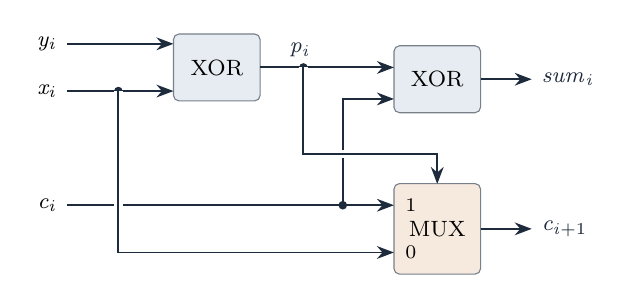
\begin{tikzpicture}[font=\footnotesize,
    gate/.style={draw=cNavy!60, rounded corners=2pt, fill=cBlue!12, minimum width=1.1cm,
                 font=\footnotesize, inner sep=0pt},
    wire/.style={->, line width=0.7pt, cNavy},
    bridge/.style={preaction={draw, white, line width=3.2pt}},
    dot/.style={circle, fill=cNavy, inner sep=1.1pt}]
  \node[gate, minimum height=0.85cm] (x1) at (1.9, 0.7) {XOR};
  \node[gate, minimum height=0.85cm] (x2) at (4.7, 0.55) {XOR};
  \node[gate, minimum height=1.15cm, fill=cOrange!16] (mx) at (4.7,-1.35) {MUX};
  \node[anchor=east] at (0, 1.0) {$y_i$};
  \node[anchor=east] at (0, 0.4) {$x_i$};
  \node[anchor=east] at (0,-1.05) {$c_i$};
  \draw[wire] (0, 1.0) -- (1.35, 1.0);
  \draw[wire] (0, 0.4) -- (1.35, 0.4);
  \draw[wire] (0,-1.05) -- (4.15,-1.05);
  \node[dot] at (3.5,-1.05) {};
  \draw[wire] (3.5,-1.05) -- (3.5, 0.3) -- (4.15, 0.3);
  \node[dot] at (0.65, 0.4) {};
  \draw[wire, bridge] (0.65, 0.4) -- (0.65,-1.65) -- (4.15,-1.65);
  \draw[wire] (2.45, 0.7) -- node[above, pos=0.3] {$p_i$} (4.15, 0.7);
  \node[dot] at (3.0, 0.7) {};
  \draw[wire, bridge] (3.0, 0.7) -- (3.0,-0.4) -- (4.7,-0.4) -- (4.7,-0.78);
  \node[font=\scriptsize, anchor=west] at (4.17,-1.05) {1};
  \node[font=\scriptsize, anchor=west] at (4.17,-1.65) {0};
  \draw[wire] (x2.east) -- (5.9, 0.55) node[right] {$\mathit{sum}_i$};
  \draw[wire] (mx.east) -- (5.9,-1.35) node[right] {$c_{i+1}$};
\end{tikzpicture}

\vspace{6pt}
\small $\mathit{sum}_i=p_i\oplus c_i$, \ $c_{i+1}=\mathrm{MUX}(p_i;c_i,x_i)$\\
\muted{4 blind rotations per bit}
\column{0.47\textwidth}
\onslide<2->{
\textbf{Example:} $5+3$ in 3 bits \muted{(LSB first)}\\[4pt]
\small
\setlength{\tabcolsep}{4pt}
\begin{tabular}{@{}cccccc@{}}
\toprule
$i$ & $x_i\,y_i$ & $c_i$ & $p_i$ & $\mathit{sum}_i$ & $c_{i+1}$\\
\midrule
0 & 1\,1 & 0 & 0 & 0 & $x_0=1$\\
1 & 0\,1 & 1 & 1 & 0 & $c_1=1$\\
2 & 1\,0 & 1 & 1 & 0 & $c_2=1$\\
\bottomrule
\end{tabular}\\[6pt]
result $1000_2=8$ \alert{\checkmark}\\[2pt]
\muted{the server runs the same 9 gates for any input}}
\end{columns}
\end{frame}

%% ===========================================================================
\section{Implementation}

\begin{frame}{Architecture: one header per layer, one test per header}
\centering
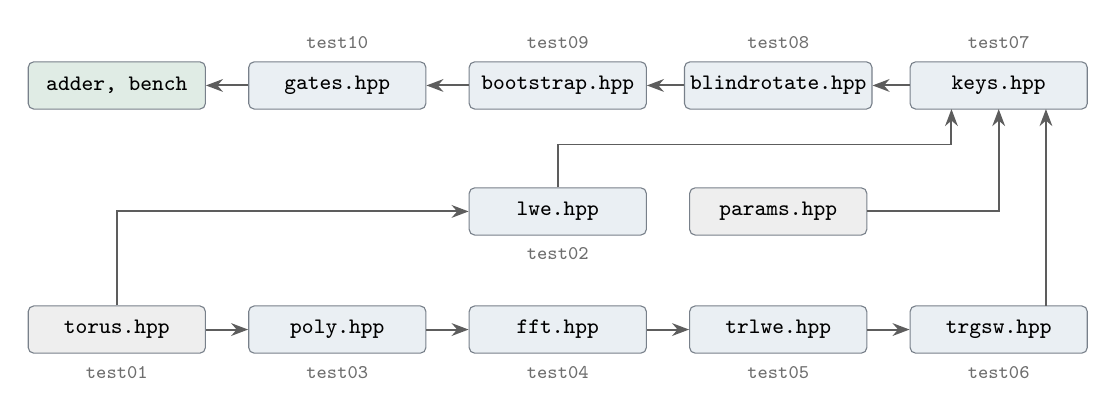
\begin{tikzpicture}[font=\footnotesize,
    dep/.style={->, cGray!85!black, line width=0.7pt},
    tst/.style={font=\scriptsize\ttfamily, cGray}]
  \node[mod=cGray!12] (torus) at (0,0) {torus.hpp};
  \node[mod] (poly)  at (2.8,0) {poly.hpp};
  \node[mod] (fft)   at (5.6,0) {fft.hpp};
  \node[mod] (trlwe) at (8.4,0) {trlwe.hpp};
  \node[mod] (trgsw) at (11.2,0) {trgsw.hpp};
  \node[mod] (lwe)   at (5.6,1.5) {lwe.hpp};
  \node[mod=cGray!12] (params) at (8.4,1.5) {params.hpp};
  \node[mod] (keys)  at (11.2,3.1) {keys.hpp};
  \node[mod] (br)    at (8.4,3.1) {blindrotate.hpp};
  \node[mod] (boot)  at (5.6,3.1) {bootstrap.hpp};
  \node[mod] (gates) at (2.8,3.1) {gates.hpp};
  \node[mod=cGreen!16] (apps) at (0,3.1) {adder, bench};
  \foreach \a/\b in {torus/poly, poly/fft, fft/trlwe, trlwe/trgsw,
                     keys/br, br/boot, boot/gates, gates/apps}
    \draw[dep] (\a) -- (\b);
  \draw[dep] (torus.north) |- (lwe.west);
  \draw[dep] (lwe.north) |- (10.6,2.35) -- (10.6,2.8);
  \draw[dep] (params.east) -| (11.2,2.8);
  \draw[dep] (11.8,0.3) -- (11.8,2.8);
  \foreach \n/\t in {torus/01, poly/03, fft/04, trlwe/05, trgsw/06} \node[tst, below=1pt of \n] {test\t};
  \node[tst, below=1pt of lwe] {test02};
  \foreach \n/\t in {keys/07, br/08, boot/09, gates/10} \node[tst, above=1pt of \n] {test\t};
\end{tikzpicture}

\vspace{8pt}
\begin{columns}[T,onlytextwidth]
\column{0.32\textwidth}\centering
\textbf{\LibLines{}} lines\\\muted{\small header-only, no dependencies}
\column{0.32\textwidth}\centering
\textbf{10} unit tests\\\muted{\small fixed seeds, independent references}
\column{0.32\textwidth}\centering
\textbf{bottom-up}\\\muted{\small no layer built on a failing test}
\end{columns}
\end{frame}

%% ===========================================================================
\begin{frame}[fragile]{Torus arithmetic in \texttt{uint32\_t}}
Three C++ rules carry the whole arithmetic:
\vspace{4pt}
\begin{enumerate}
  \item \textbf{Unsigned arithmetic is mod $2^{32}$} \muted{-- exactly the torus.
        Signed overflow is undefined behavior: an optimizer may break it.}
  \item<2-> \textbf{\texttt{k * t} converts \texttt{k} to unsigned} \muted{--
        still correct mod $2^{32}$ for negative $k$.}
  \item<3-> \textbf{\texttt{int32\_t(t)} rereads the bits as signed}
        \muted{-- the representative in $[-\frac12,\frac12)$: how noise is measured
        and how a bit is decrypted.}
\end{enumerate}
\vspace{6pt}
\begin{uncoverenv}<4->
\begin{columns}[T,onlytextwidth]
\column{0.46\textwidth}
\begin{lstlisting}[basicstyle=\ttfamily\scriptsize]
using Torus = uint32_t;
// decrypt a bit: sign of the phase
bool bit = int32_t(lwePhase(c, s)) > 0;
\end{lstlisting}
\column{0.5\textwidth}
\begin{lstlisting}[basicstyle=\ttfamily\scriptsize]
// round t to Z_2N: product in 64 bits,
// add 1/2, drop the 32 low bits
(uint64_t(t) * twoN + (1ull << 31)) >> 32
\end{lstlisting}
\end{columns}
\end{uncoverenv}
\end{frame}

%% ===========================================================================
\begin{frame}{Why evaluate at the roots of $X^N+1$?}
\begin{columns}[c,onlytextwidth]
\column{0.4\textwidth}
\centering
% Roots of X^8 + 1 on the unit circle: the four evaluation points of the
% negacyclic FFT and their conjugates. Shared by the report and the slides.
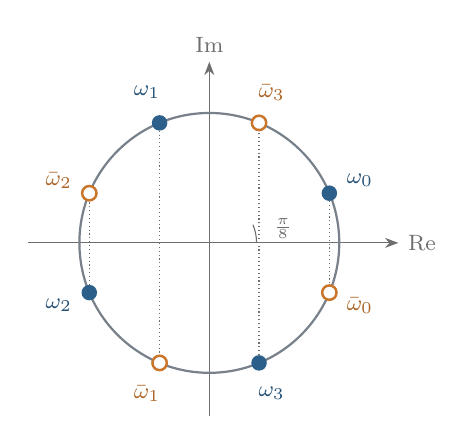
\begin{tikzpicture}[font=\footnotesize, >=Stealth]
  \def\rad{1.65}
  \draw[->, cGray] (-2.3,0) -- (2.4,0) node[right] {Re};
  \draw[->, cGray] (0,-2.2) -- (0,2.3) node[above] {Im};
  \draw[cNavy!60, line width=0.8pt] (0,0) circle (\rad);
  \foreach \a/\b in {22.5/337.5, 112.5/247.5, 202.5/157.5, 292.5/67.5}
    \draw[cGray, densely dotted] (\a:\rad) -- (\b:\rad);
  \foreach \a/\k in {22.5/0, 112.5/1, 202.5/2, 292.5/3} {
    \fill[cBlue] (\a:\rad) circle (2.8pt);
    \node[cBlue!85!black] at (\a:\rad+0.42) {$\omega_{\k}$};
  }
  \foreach \a/\k in {337.5/0, 247.5/1, 157.5/2, 67.5/3} {
    \draw[cOrange, fill=white, line width=0.9pt] (\a:\rad) circle (2.6pt);
    \node[cOrange!85!black] at (\a:\rad+0.42) {$\bar\omega_{\k}$};
  }
  \draw[cGray] (0.6,0) arc (0:22.5:0.6);
  \node[cGray, font=\scriptsize] at (11:0.95) {$\frac{\pi}{8}$};
\end{tikzpicture}
\\[2pt]
\footnotesize roots of $X^8+1$: we use $\omega_0,\dots,\omega_3$;\\
the others are their conjugates.
\column{0.58\textwidth}
At a root, $\omega^N=-1$: \alert{the reduction mod $X^N+1$ is automatic}.

\vspace{6pt}
\onslide<2->{
\textbf{Example} ($N=4$): $a=1+X$, $b=X^3$, \ $a\cdot b=-1+X^3$\\[4pt]
\small
\setlength{\tabcolsep}{5pt}
\begin{tabular}{@{}lcc@{}}
\toprule
 & $\omega_0=e^{i\pi/4}$ & $\omega_1=e^{i5\pi/4}$\\
\midrule
$a(\omega)$ & $1.707+0.707i$ & $0.293-0.707i$\\
$b(\omega)$ & $-0.707+0.707i$ & $0.707-0.707i$\\
$a(\omega)\,b(\omega)$ & $-1.707+0.707i$ & $-0.293-0.707i$\\
\uncover<3->{$-1+\omega^3$} & \uncover<3->{\alert{$-1.707+0.707i$}} & \uncover<3->{\alert{$-0.293-0.707i$}}\\
\bottomrule
\end{tabular}}
\onslide<3->{\\[4pt]\small $N$ products instead of $N^2$, \ \muted{plus the cost of the transforms}}
\end{columns}
\end{frame}

%% ===========================================================================
\begin{frame}{Negacyclic FFT: fold and twist}
\centering
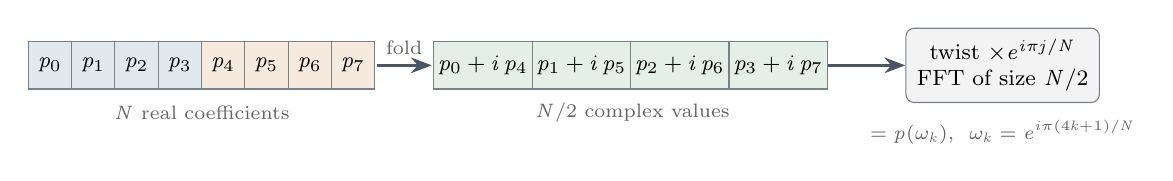
\begin{tikzpicture}[font=\footnotesize,
    fstep/.style={->, line width=1pt, cNavy!80},
    note/.style={font=\scriptsize, align=center, cGray!90!black}]
  \foreach \j in {0,...,3} \node[cellF=cBlue!14] at (\j*0.55, 0) {$p_{\j}$};
  \foreach \j in {4,...,7} \node[cellF=cOrange!16] at (\j*0.55, 0) {$p_{\j}$};
  \node[note] at (1.93,-0.6) {$N$ real coefficients};
  \draw[fstep] (4.15,0) -- node[above, note] {fold} (4.85,0);
  \foreach \j in {0,...,3} {\pgfmathtruncatemacro{\k}{\j+4}
    \node[cellF=cGreen!14, minimum width=1.25cm] (z\j) at (5.5+\j*1.25, 0) {$p_{\j}+i\,p_{\k}$};}
  \node[note] at (7.4,-0.6) {$N/2$ complex values};
  \node[draw=cNavy!60, rounded corners=3pt, fill=cGray!8, align=center, inner sep=4pt]
    (tw) at (12.1,0) {twist $\times e^{i\pi j/N}$\\FFT of size $N/2$};
  \draw[fstep] (z3.east) -- (tw.west);
  \node[note] at (12.1,-0.85) {$=p(\omega_k)$, \ $\omega_k=e^{i\pi(4k+1)/N}$};
\end{tikzpicture}

\vspace{12pt}
\begin{columns}[T,onlytextwidth]
\column{0.5\textwidth}
\begin{itemize}
  \item Evaluate at roots of $X^N+1$: the reduction \alert{happens by itself}.
  \item Real coefficients: one root per conjugate pair suffices.
  \item Radix-2 Cooley--Tukey, tables precomputed once.
  \item Hand-written \texttt{cmul}: \texttt{std::complex} checks NaN/$\infty$.
\end{itemize}
\column{0.46\textwidth}
\onslide<2->{
\begin{block}{Is \texttt{double} precise enough?}
digit $\cdot$ torus $\cdot$ $N$ terms:
$2^{6}\cdot2^{31}\cdot2^{10}=2^{47}<2^{53}$\\[3pt]
measured: \alert{bit-exact}, and $\FftSpeedup\times$ faster than schoolbook
\muted{(\FftNaive\,\textmu s $\to$ \FftFast\,\textmu s)}
\end{block}}
\end{columns}
\end{frame}

%% ===========================================================================
\begin{frame}{The offset trick (1/2): balanced digits with one addition}
\begin{itemize}
  \item $2N\ell=6144$ digits per external product: decomposition must be cheap.
  \item Unsigned digits $[0,\Bg)$ are bit fields, but \alert{balanced} digits
        $[-\frac{\Bg}2,\frac{\Bg}2)$ halve $\beta$: \alert{$4\times$ less} noise.
  \item Converting needs carry propagation \emph{and} rounding.
\end{itemize}
\vspace{2pt}
\onslide<2->{
\begin{block}{Lemma (offset trick)}
With $h_i=2^{32-7i}$ and
$\mathit{offset}=\sum_{i=1}^{\ell}\frac{\Bg}{2}h_i+\frac{h_\ell}{2}$:
take the bit fields $u_i$ of $t+\mathit{offset}$, set $d_i=u_i-\frac{\Bg}{2}$. Then
\[t=\sum_i d_ih_i+\underbrace{(r-h_\ell/2)}_{|\cdot|\,\le\,\varepsilon}\pmod{2^{32}}.\]
\end{block}}
\onslide<3->{\small\muted{Proof: write $t+\mathit{offset}=\sum_iu_ih_i+r$ and subtract.}
\quad Base 10: $\mathit{offset}=0.555$, \ $0.7316+0.555\equiv0.2866\Rightarrow(2,8)-5=(-3,3)$.}
\end{frame}

%% ===========================================================================
\begin{frame}[fragile]{The offset trick (2/2): $t=0.7$, \ $\Bg=2^7$, \ $\ell=3$}
\centering
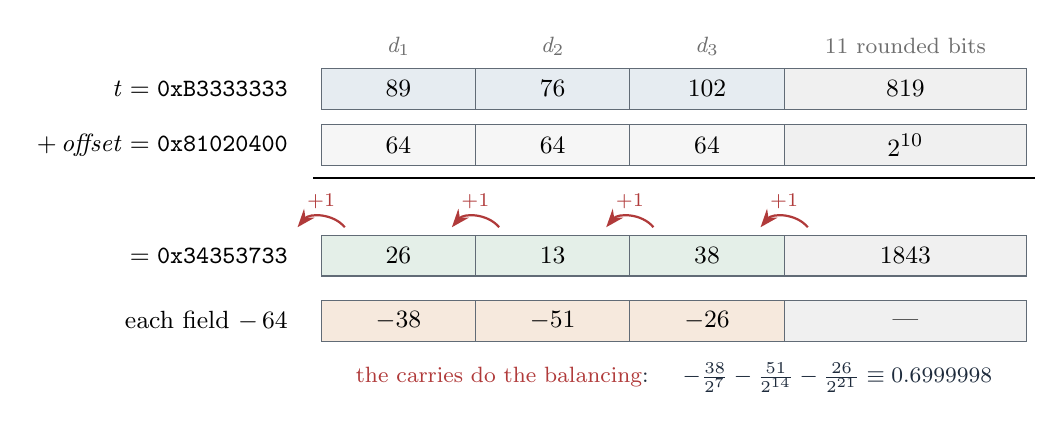
\begin{tikzpicture}[font=\small]
  \def\u{0.28}
  \def\h{0.52}
  \newcommand{\word}[7]{%
    \begin{scope}[visible on=#7]
    \fill[#2] (0,#1) rectangle (21*\u,#1+\h);
    \fill[cGray!10] (21*\u,#1) rectangle (32*\u,#1+\h);
    \draw[cNavy!70] (0,#1) rectangle (32*\u,#1+\h);
    \foreach \b in {7,14,21} \draw[cNavy!70] (\b*\u,#1) -- (\b*\u,#1+\h);
    \node at (3.5*\u,#1+0.5*\h) {#3};
    \node at (10.5*\u,#1+0.5*\h) {#4};
    \node at (17.5*\u,#1+0.5*\h) {#5};
    \node at (26.5*\u,#1+0.5*\h) {#6};
    \end{scope}
  }
  \node[cGray, font=\footnotesize] at (3.5*\u, 0.8) {$d_1$};
  \node[cGray, font=\footnotesize] at (10.5*\u,0.8) {$d_2$};
  \node[cGray, font=\footnotesize] at (17.5*\u,0.8) {$d_3$};
  \node[cGray, font=\footnotesize] at (26.5*\u,0.8) {11 rounded bits};
  \word{0}{cBlue!12}{$89$}{$76$}{$102$}{$819$}{<1->}
  \word{-0.72}{cGray!6}{$64$}{$64$}{$64$}{$2^{10}$}{<2->}
  \draw[visible on=<3->, line width=0.7pt] (-0.1,-0.88) -- (32*\u+0.1,-0.88);
  \foreach \b in {21,14,7,0} {
    \draw[visible on=<3->, ->, cRed, line width=0.8pt] (\b*\u+0.3,-1.5) to[bend right=50]
      node[above=-1pt, font=\scriptsize] {$+1$} (\b*\u-0.3,-1.5);
  }
  \word{-2.12}{cGreen!14}{$26$}{$13$}{$38$}{$1843$}{<3->}
  \word{-2.95}{cOrange!16}{$-38$}{$-51$}{$-26$}{---}{<4->}
  \begin{scope}[every node/.style={anchor=east, font=\small}]
    \node at (-0.3, 0.26) {$t=\texttt{0xB3333333}$};
    \node[visible on=<2->] at (-0.3,-0.46) {$+\,\mathit{offset}=\texttt{0x81020400}$};
    \node[visible on=<3->] at (-0.3,-1.86) {$=\texttt{0x34353733}$};
    \node[visible on=<4->] at (-0.3,-2.69) {each field $-\,64$};
  \end{scope}
  \node[visible on=<4->, anchor=north, font=\footnotesize] at (16*\u,-3.1)
    {\color{cRed}the carries do the balancing\color{cNavy}: \quad
     $-\frac{38}{2^7}-\frac{51}{2^{14}}-\frac{26}{2^{21}}\equiv0.6999998$};
\end{tikzpicture}

\vspace{6pt}
\begin{uncoverenv}<5->
\begin{lstlisting}[basicstyle=\ttfamily\footnotesize]
uint32_t t = p[j] + g.offset;                              // the only addition
for (int i = 0; i < g.ell; ++i)
    out[i][j] = int32_t((t >> (32-(i+1)*g.Bgbit)) & g.mask) - int32_t(g.halfBg);
\end{lstlisting}
\end{uncoverenv}
\end{frame}

%% ===========================================================================
\begin{frame}{External product in the frequency domain}
\centering
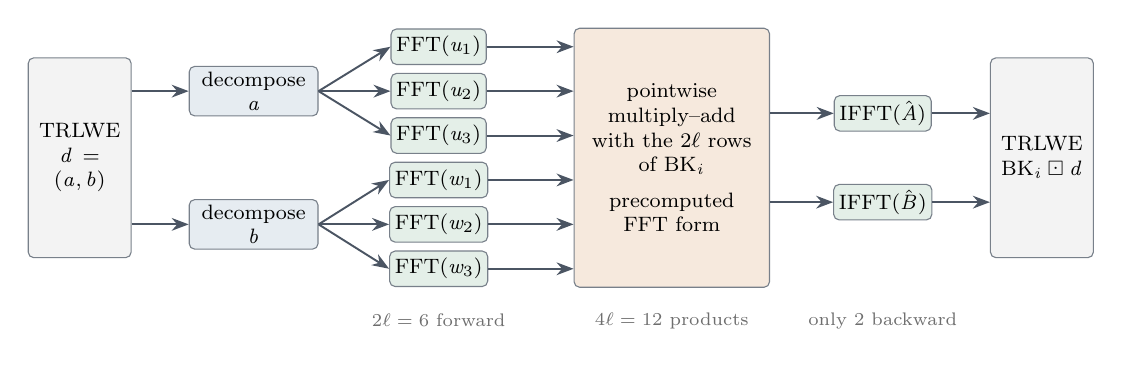
\begin{tikzpicture}[font=\footnotesize, scale=0.94, transform shape,
    flow/.style={->, line width=0.7pt, cNavy!80}]
  \node[box=cGray!8, minimum height=2.7cm, text width=1.25cm] (d) at (0,0) {TRLWE\\$d=(a,b)$};
  \node[box=cBlue!12, text width=1.6cm] (deca) at (2.35, 0.9) {decompose $a$};
  \node[box=cBlue!12, text width=1.6cm] (decb) at (2.35,-0.9) {decompose $b$};
  \draw[flow] (d.east |- deca) -- (deca);
  \draw[flow] (d.east |- decb) -- (decb);
  \foreach \i/\y in {1/1.5, 2/0.9, 3/0.3} {
    \node[box=cGreen!14] (fu\i) at (4.85,\y) {FFT$(u_{\i})$};
    \draw[flow] (deca.east) -- (fu\i.west);}
  \foreach \i/\y in {1/-0.3, 2/-0.9, 3/-1.5} {
    \node[box=cGreen!14] (fw\i) at (4.85,\y) {FFT$(w_{\i})$};
    \draw[flow] (decb.east) -- (fw\i.west);}
  \node[box=cOrange!16, minimum height=3.5cm, text width=2.5cm] (mac) at (8.0,0)
    {pointwise\\multiply--add\\with the $2\ell$ rows\\of $\BK_i$\\[4pt]
     \alert{precomputed}\\\alert{FFT form}};
  \foreach \n in {fu1,fu2,fu3,fw1,fw2,fw3} \draw[flow] (\n.east) -- (\n.east -| mac.west);
  \node[box=cGreen!14] (ia) at (10.85, 0.6) {IFFT$(\hat A)$};
  \node[box=cGreen!14] (ib) at (10.85,-0.6) {IFFT$(\hat B)$};
  \draw[flow] (mac.east |- ia) -- (ia);
  \draw[flow] (mac.east |- ib) -- (ib);
  \node[box=cGray!8, minimum height=2.7cm, text width=1.25cm] (r) at (13.0,0) {TRLWE\\$\BK_i\ext d$};
  \draw[flow] (ia.east) -- (ia.east -| r.west);
  \draw[flow] (ib.east) -- (ib.east -| r.west);
  \node[font=\scriptsize, cGray] at (4.85,-2.2) {$2\ell=6$ forward};
  \node[font=\scriptsize, cGray] at (8.0,-2.2) {$4\ell=12$ products};
  \node[font=\scriptsize, cGray] at (10.85,-2.2) {only $2$ backward};
\end{tikzpicture}

\vspace{8pt}
\onslide<2->{
$8$ FFTs per external product $\times$ $630$ per gate $\approx$ \alert{5000 FFTs of size 512 per gate}.\\
\muted{Price: $\BK$ takes \BkMB\,MiB, twice its coefficient form.}}
\end{frame}

%% ===========================================================================
\section{Evaluation}

\begin{frame}{Setup and correctness}
\begin{columns}[T,onlytextwidth]
\column{0.48\textwidth}
\textbf{Setup}
\begin{itemize}
  \item \CPU, one thread pinned to a performance core.
  \item \Compiler, \texttt{-O3 -march=native}.
  \item Original library, two FFT back ends:\\
        \textbf{spqlios-fma} \muted{(AVX2/FMA assembly)},\\
        \textbf{nayuki-portable} \muted{(plain C)}.
  \item \OurRuns{}/\OrigRuns{} runs (ours/original), $500$ gates each.
\end{itemize}
\column{0.48\textwidth}
\onslide<2->{
\textbf{Correctness}
\begin{itemize}
  \item All 10 unit tests pass; 50 chained NANDs; majority circuit.
  \item Adder: \AdderEightText{} in \AdderEight\,s, \AdderTwentyFourText{} in \AdderTwentyFour\,s.
  \item \alert{0 decryption errors in \TotalGates{} gates}.
\end{itemize}}
\onslide<3->{
\begin{exampleblock}{Why no errors?}
Input std.\ dev.\ $\approx0.005$ vs.\ margin $\frac18$: \textbf{over 20 std.\ devs.}
\end{exampleblock}}
\end{columns}
\end{frame}

%% ===========================================================================
\begin{frame}{Performance against the original library}
\begin{columns}[c,onlytextwidth]
\column{0.5\textwidth}
\centering
\begin{tikzpicture}
\begin{axis}[ybar, bar width=0.85cm, width=7.2cm, height=5.9cm, ymin=0, ymax=135,
    xtick={0,1,2}, xticklabels={{this work},{spqlios-fma},{nayuki}},
    tick label style={font=\footnotesize}, ylabel={ms per NAND gate},
    label style={font=\small}, enlarge x limits=0.25, ymajorgrids,
    grid style={cGray!20}, axis line style={cGray},
    point meta=explicit symbolic,
    nodes near coords={\pgfmathprintnumber[fixed,zerofill,precision=1]{\pgfplotspointmeta}},
    nodes near coords style={font=\small\bfseries, anchor=south}]
  \addplot[fill=cOrange!80, draw=cOrange!80!black]
    table[x=x, y=nand, meta=nand, restrict expr to domain={\coordindex}{0:0}] {../report/data/time.dat};
  \addplot[fill=cBlue!45, draw=cBlue]
    table[x=x, y=nand, meta=nand, restrict expr to domain={\coordindex}{1:2}] {../report/data/time.dat};
\end{axis}
\end{tikzpicture}
\column{0.48\textwidth}
\begin{itemize}
  \item \alert{$\SlowdownSpq\times$ slower} than the assembly FFT.
  \item \alert{$\SpeedupNay\times$ faster} than the portable FFT.
  \item[$\Rightarrow$] Same algorithm in all three: the \textbf{FFT decides}.
\end{itemize}
\vspace{6pt}
\onslide<2->{
\footnotesize\setlength{\tabcolsep}{3.5pt}
\begin{tabular}{@{}lccc@{}}
\toprule
 & ours & spqlios & nayuki\\
\midrule
key gen.\ (s) & \OurKeygenRange & \SpqKeygenRange & \NayKeygenRange\\
peak mem.\ (MiB) & \OurRSS & \SpqRSS & \NayRSS\\
\bottomrule
\end{tabular}\\[4pt]
\muted{\footnotesize Keys: $\BK$ \BkMB\,MiB, $\KSK$ \KskMB\,MiB; one encrypted bit: 2524 bytes.}}
\end{columns}
\end{frame}

%% ===========================================================================
\begin{frame}{Where the time goes}
\begin{columns}[c,onlytextwidth]
\column{0.56\textwidth}
\centering
\begin{tikzpicture}
\begin{axis}[xbar, bar width=0.36cm, width=6.0cm, height=6.4cm,
    xmin=0, xmax=7.6, enlarge y limits=0.09, xlabel={ms per gate},
    ytick={0,...,6},
    yticklabels={{decomposition}, {rotation, add/sub}, {key switching},
                 {other}, {backward FFTs}, {pointwise products}, {forward FFTs}},
    tick label style={font=\footnotesize}, label style={font=\small},
    xmajorgrids, grid style={cGray!20}, axis line style={cGray},
    point meta=explicit symbolic,
    nodes near coords={\pgfmathprintnumber[fixed,precision=0]{\pgfplotspointmeta}\%},
    nodes near coords style={font=\scriptsize, anchor=west}]
  \addplot[fill=cBlue!55, draw=cBlue] table[x=ms, y=y, meta=pct] {../report/data/profile.dat};
\end{axis}
\end{tikzpicture}
\column{0.42\textwidth}
\begin{itemize}
  \item Blind rotation: \BRShare\% of the gate.
  \item FFTs + pointwise products: \alert{\FreqShare\%}.
  \item Decomposition: only \DecShare\% \muted{(offset trick)}.
\end{itemize}
\onslide<2->{
\begin{alertblock}{Surprise: memory traffic}
\small Each step reads a different $\BK_i$: the \BkMB\,MiB key is
\emph{streamed} every gate.\\[3pt]
External product: \ExtHot\,\textmu s (key in cache) vs.\
\alert{\ExtKey\,\textmu s} (as in blind rotation) $\approx$ \MemShare\% of the gate.
\end{alertblock}}
\end{columns}
\end{frame}

%% ===========================================================================
\begin{frame}{Noise: bounds, predictions and measurements}
\begin{columns}[c,onlytextwidth]
\column{0.5\textwidth}
\begin{itemize}
  \item Worst-case bounds assume every digit has magnitude $\beta$.
  \item Digits are \alert{uniform}: $\mathbb E[d^2]\approx\beta^2/3$ $\Rightarrow$ a third of the bound.
  \item<2-> Key switching: fixed table noise, only $\frac34$ of digits nonzero.
\end{itemize}
\vspace{4pt}
\onslide<3->{
\small\setlength{\tabcolsep}{3.5pt}
\begin{tabular}{@{}lccc@{}}
\toprule
variance & bound & predicted & measured\\
\midrule
blind rot. & \BoundBR & \AvgBR & \alert{\NoiseVarBR}\\
gate output & \BoundTotal & \AvgTotal & \alert{\NoiseVarKS}\\
\bottomrule
\end{tabular}\\[3pt]
\muted{\footnotesize \NoiseKeys{} keys $\times$ \NoiseGates{} gates, within-key variance}}
\column{0.48\textwidth}
\onslide<3->{
\centering
\begin{tikzpicture}
\begin{axis}[width=7.0cm, height=5.6cm, xmin=-12, xmax=12, ymin=0,
    xlabel={error $-$ key mean ($10^{-3}$)}, ytick=\empty,
    tick label style={font=\footnotesize}, label style={font=\small},
    axis line style={cGray}, scaled ticks=false,
    legend style={font=\scriptsize, at={(0.98,0.97)}, anchor=north east, draw=none,
                  fill=white, fill opacity=0.85, text opacity=1},
    legend cell align=left]
  \addplot[ybar interval=0.98, fill=cBlue!35, draw=cBlue!70!black]
    table[x expr=\thisrow{center}*1000-0.25, y=density] {../report/data/noise_hist.dat};
  \addlegendentry{measured}
  \addplot[cOrange, line width=1.4pt, domain=-12:12, samples=161]
    {exp(-(x/1000)^2/(2*\AvgTotalRaw))/sqrt(2*pi*\AvgTotalRaw)};
  \addlegendentry{prediction}
\end{axis}
\end{tikzpicture}}
\end{columns}
\end{frame}

%% ===========================================================================
\begin{frame}{A key-dependent bias, and why the original has none}
\begin{columns}[c,onlytextwidth]
\column{0.5\textwidth}
\begin{itemize}
  \item Each $\KSK$ entry carries a \alert{fixed} noise $e_{i,j,v}$.
  \item Averaging over inputs with the table fixed leaves a per-key
        \alert{bias}:
        \[\mathrm{std}\approx\sqrt{3tN/16}\;\sigma_{\mathrm{LWE}}=\BiasStd\]
  \item<2-> Measured over \NoiseKeys{} keys: \alert{\NoiseBiasStd}.
  \item<3-> The original library \textbf{centers} its key-switching noise
        $\Rightarrow$ mean error $\le\SpqMeanMax$ vs.\ ours up to \OurMeanMax.
  \item<3-> Harmless: $100\times$ below the margin.
\end{itemize}
\column{0.48\textwidth}
\centering
\begin{tikzpicture}
\begin{axis}[width=7.0cm, height=5.6cm, xmin=0.3, xmax=10.7, ymin=-3.2, ymax=3.2,
    xtick={1,...,10}, xlabel={key}, ylabel={mean error ($10^{-3}$)},
    tick label style={font=\footnotesize}, label style={font=\small},
    axis line style={cGray}, ymajorgrids, grid style={cGray!20}]
  \fill[cOrange!12] (axis cs:0.3,{-2000*\BiasStdRaw}) rectangle (axis cs:10.7,{2000*\BiasStdRaw});
  \fill[cOrange!25] (axis cs:0.3,{-1000*\BiasStdRaw}) rectangle (axis cs:10.7,{1000*\BiasStdRaw});
  \draw[cGray, densely dashed] (axis cs:0.3,0) -- (axis cs:10.7,0);
  \addplot[only marks, mark=*, mark size=2.6pt, cBlue,
           visible on=<2->]
    table[x=key, y expr=\thisrow{meanKS}*1000] {../report/data/noise_keys.dat};
  \node[font=\scriptsize, cOrange!80!black, anchor=north east] at (axis cs:10.6,3.1)
    {bands: $\pm1\sigma$, $\pm2\sigma$ predicted};
\end{axis}
\end{tikzpicture}
\end{columns}
\end{frame}

%% ===========================================================================
\begin{frame}{Limitations and future work}
\begin{columns}[T,onlytextwidth]
\column{0.47\textwidth}
\textbf{Limitations}
\begin{itemize}
  \item \texttt{mt19937\_64} is \alert{not} a CSPRNG.
  \item No constant-time guarantees on the client.
  \item No serialization: client and server share a process.
  \item Parameters: $\approx128$ bits as estimated by the library authors;
        re-check with a current lattice estimator.
\end{itemize}
\column{0.5\textwidth}
\textbf{Next steps} \muted{(by expected gain per effort)}
\begin{enumerate}
  \item Center the key-switching noise.
  \item Remove allocations from the inner loops.
  \item Contiguous $\BK$ + prefetch the next TRGSW sample.
  \item Vectorize the FFT (AVX2/FMA) or radix-4.
  \item Independent gates in parallel threads.
  \item Programmable bootstrapping.
\end{enumerate}
\end{columns}
\end{frame}

%% ===========================================================================
\begin{frame}{Takeaways}
\centering
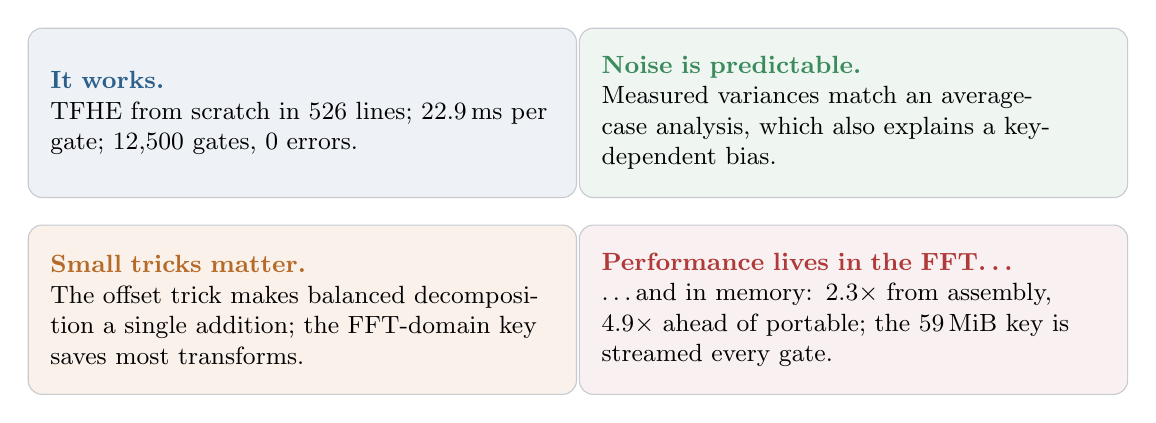
\begin{tikzpicture}[font=\small,
]
  \node[card=cBlue!8] at (0,1.25) {\textbf{\color{cBlue}It works.}\\
    TFHE from scratch in \LibLines{} lines; \OurNandMean\,ms per gate;
    \TotalGates{} gates, 0 errors.};
  \node[card=cGreen!8] at (7.0,1.25) {\textbf{\color{cGreen}Noise is predictable.}\\
    Measured variances match an average-case analysis, which also explains a
    key-dependent bias.};
  \node[card=cOrange!10] at (0,-1.25) {\textbf{\color{cOrange!90!black}Small tricks matter.}\\
    The offset trick makes balanced decomposition a single addition; the
    FFT-domain key saves most transforms.};
  \node[card=cRed!7] at (7.0,-1.25) {\textbf{\color{cRed}Performance lives in the FFT\dots}\\
    \dots and in memory: $\SlowdownSpq\times$ from assembly, $\SpeedupNay\times$
    ahead of portable; the 59\,MiB key is streamed every gate.};
\end{tikzpicture}
\end{frame}

%% ===========================================================================
{
\setbeamercolor{background canvas}{bg=cNavy}
\begin{frame}[plain]
\centering
\vspace{1.2cm}
{\color{white}\Huge Thank you!}\\[14pt]
{\color{cOrange}\Large Questions?}\\[30pt]
{\color{white!75}\small Matheus de Oliveira Saldanha \textbullet\ MO422 \textbullet\ Unicamp}\\[4pt]
{\color{white!60}\footnotesize code, tests, report and these slides: \texttt{learning-tfhe}}
\end{frame}
}

%% ===========================================================================
\appendix

\begin{frame}{Backup: parameters}
\centering
\begin{tabular}{@{}lll@{}}
\toprule
Symbol & Value & Role\\
\midrule
$n$ & $630$ & LWE dimension; external products per bootstrapping\\
$N$ & $1024$ & ring degree; the phase is rounded to $2N$ positions\\
$\ell$, $\Bg$ & $3$, $2^7$ & gadget decomposition of the external product\\
$t$, base & $8$, $2^2$ & decomposition of the key switching\\
$\sigma_{\mathrm{LWE}}$ & $2^{-15}$ & noise of LWE samples and of $\KSK$\\
$\sigma_{\BK}$ & $2^{-25}$ & noise of the TRGSW samples of $\BK$\\
\bottomrule
\end{tabular}

\vspace{10pt}
\small The same as \texttt{new\_default\_gate\_bootstrapping\_parameters(128)} of the original library.
\end{frame}

\begin{frame}{Backup: noise of a bootstrapped gate}
\centering
\small
\renewcommand{\arraystretch}{1.6}
\begin{tabular}{@{}lll@{}}
\toprule
 & worst-case bound & average case\\
\midrule
blind rotation & $n\big(2\ell N\beta^2\vartheta_{\BK}+(1+N)\varepsilon^2\big)=\BoundBR$
  & $n\,2\ell N\frac{\beta^2}{3}\vartheta_{\BK}=\AvgBR$\\
key switching & $tN\vartheta_{\KSK}+N\,2^{-2(t\cdot\mathrm{basebit}+1)}$
  & $tN\big(\frac{B-1}{B}\big)^2\vartheta_{\KSK}=\AvgKS$\\
per-key bias & --- & $\sqrt{tN\frac{B-1}{B^2}\vartheta_{\KSK}}=\BiasStd$ \ (std.)\\
rounding to $\Z_{2N}$ & \multicolumn{2}{l}{$\frac{1+n/2}{48N^2}\approx6.3\cdot10^{-6}$ \ (input side only)}\\
\bottomrule
\end{tabular}

\vspace{10pt}
NAND input: two gate outputs + rounding $\Rightarrow$ $\sigma\approx0.005\ll\frac18$.
\end{frame}

\end{document}
